\documentclass[twoside]{book}

% Packages required by doxygen
\usepackage{fixltx2e}
\usepackage{calc}
\usepackage{doxygen}
\usepackage[export]{adjustbox} % also loads graphicx
\usepackage{graphicx}
\usepackage[utf8]{inputenc}
\usepackage{makeidx}
\usepackage{multicol}
\usepackage{multirow}
\PassOptionsToPackage{warn}{textcomp}
\usepackage{textcomp}
\usepackage[nointegrals]{wasysym}
\usepackage[table]{xcolor}

% Font selection
\usepackage[T1]{fontenc}
\usepackage[scaled=.90]{helvet}
\usepackage{courier}
\usepackage{amssymb}
\usepackage{sectsty}
\renewcommand{\familydefault}{\sfdefault}
\allsectionsfont{%
  \fontseries{bc}\selectfont%
  \color{darkgray}%
}
\renewcommand{\DoxyLabelFont}{%
  \fontseries{bc}\selectfont%
  \color{darkgray}%
}
\newcommand{\+}{\discretionary{\mbox{\scriptsize$\hookleftarrow$}}{}{}}

% Page & text layout
\usepackage{geometry}
\geometry{%
  a4paper,%
  top=2.5cm,%
  bottom=2.5cm,%
  left=2.5cm,%
  right=2.5cm%
}
\tolerance=750
\hfuzz=15pt
\hbadness=750
\setlength{\emergencystretch}{15pt}
\setlength{\parindent}{0cm}
\setlength{\parskip}{3ex plus 2ex minus 2ex}
\makeatletter
\renewcommand{\paragraph}{%
  \@startsection{paragraph}{4}{0ex}{-1.0ex}{1.0ex}{%
    \normalfont\normalsize\bfseries\SS@parafont%
  }%
}
\renewcommand{\subparagraph}{%
  \@startsection{subparagraph}{5}{0ex}{-1.0ex}{1.0ex}{%
    \normalfont\normalsize\bfseries\SS@subparafont%
  }%
}
\makeatother

% Headers & footers
\usepackage{fancyhdr}
\pagestyle{fancyplain}
\fancyhead[LE]{\fancyplain{}{\bfseries\thepage}}
\fancyhead[CE]{\fancyplain{}{}}
\fancyhead[RE]{\fancyplain{}{\bfseries\leftmark}}
\fancyhead[LO]{\fancyplain{}{\bfseries\rightmark}}
\fancyhead[CO]{\fancyplain{}{}}
\fancyhead[RO]{\fancyplain{}{\bfseries\thepage}}
\fancyfoot[LE]{\fancyplain{}{}}
\fancyfoot[CE]{\fancyplain{}{}}
\fancyfoot[RE]{\fancyplain{}{\bfseries\scriptsize Generated by Doxygen }}
\fancyfoot[LO]{\fancyplain{}{\bfseries\scriptsize Generated by Doxygen }}
\fancyfoot[CO]{\fancyplain{}{}}
\fancyfoot[RO]{\fancyplain{}{}}
\renewcommand{\footrulewidth}{0.4pt}
\renewcommand{\chaptermark}[1]{%
  \markboth{#1}{}%
}
\renewcommand{\sectionmark}[1]{%
  \markright{\thesection\ #1}%
}

% Indices & bibliography
\usepackage{natbib}
\usepackage[titles]{tocloft}
\setcounter{tocdepth}{3}
\setcounter{secnumdepth}{5}
\makeindex

% Hyperlinks (required, but should be loaded last)
\usepackage{ifpdf}
\ifpdf
  \usepackage[pdftex,pagebackref=true]{hyperref}
\else
  \usepackage[ps2pdf,pagebackref=true]{hyperref}
\fi
\hypersetup{%
  colorlinks=true,%
  linkcolor=blue,%
  citecolor=blue,%
  unicode%
}

% Custom commands
\newcommand{\clearemptydoublepage}{%
  \newpage{\pagestyle{empty}\cleardoublepage}%
}

\usepackage{caption}
\captionsetup{labelsep=space,justification=centering,font={bf},singlelinecheck=off,skip=4pt,position=top}

%===== C O N T E N T S =====

\begin{document}

% Titlepage & ToC
\hypersetup{pageanchor=false,
             bookmarksnumbered=true,
             pdfencoding=unicode
            }
\pagenumbering{alph}
\begin{titlepage}
\vspace*{7cm}
\begin{center}%
{\Large Rookie Tales \\[1ex]\large 2.\+0 }\\
\vspace*{1cm}
{\large Generated by Doxygen 1.8.13}\\
\end{center}
\end{titlepage}
\clearemptydoublepage
\pagenumbering{roman}
\tableofcontents
\clearemptydoublepage
\pagenumbering{arabic}
\hypersetup{pageanchor=true}

%--- Begin generated contents ---
\chapter{Data Structure Index}
\section{Data Structures}
Here are the data structures with brief descriptions\+:\begin{DoxyCompactList}
\item\contentsline{section}{\hyperlink{structBackground}{Background} }{\pageref{structBackground}}{}
\item\contentsline{section}{\hyperlink{structbackground}{background} \\*For background }{\pageref{structbackground}}{}
\item\contentsline{section}{\hyperlink{structBoss}{Boss} \\*\hyperlink{structBoss}{Boss} stuct }{\pageref{structBoss}}{}
\item\contentsline{section}{\hyperlink{structButton}{Button} \\*For loading a button }{\pageref{structButton}}{}
\item\contentsline{section}{\hyperlink{structcharacter}{character} \\*For character choice }{\pageref{structcharacter}}{}
\item\contentsline{section}{\hyperlink{structChoice}{Choice} \\*To account for the choice }{\pageref{structChoice}}{}
\item\contentsline{section}{\hyperlink{structchoice__button}{choice\+\_\+button} \\*To update buttons in the menu }{\pageref{structchoice__button}}{}
\item\contentsline{section}{\hyperlink{structDialogue}{Dialogue} \\*To load the dialogue in the game }{\pageref{structDialogue}}{}
\item\contentsline{section}{\hyperlink{structDirection}{Direction} \\*Describe the hero direction }{\pageref{structDirection}}{}
\item\contentsline{section}{\hyperlink{structenigme}{enigme} \\*Struct for the enigma }{\pageref{structenigme}}{}
\item\contentsline{section}{\hyperlink{structEntite}{Entite} \\*General entity struct }{\pageref{structEntite}}{}
\item\contentsline{section}{\hyperlink{structetat}{etat} \\*For the game state }{\pageref{structetat}}{}
\item\contentsline{section}{\hyperlink{structheart}{heart} \\*\hyperlink{structHeart}{Heart} you collect }{\pageref{structheart}}{}
\item\contentsline{section}{\hyperlink{structHeart}{Heart} }{\pageref{structHeart}}{}
\item\contentsline{section}{\hyperlink{structHero}{Hero} \\*Anything used by the main character }{\pageref{structHero}}{}
\item\contentsline{section}{\hyperlink{structHeure}{Heure} }{\pageref{structHeure}}{}
\item\contentsline{section}{\hyperlink{structheure}{heure} \\*For time }{\pageref{structheure}}{}
\item\contentsline{section}{\hyperlink{structMat}{Mat} }{\pageref{structMat}}{}
\item\contentsline{section}{\hyperlink{structMatchstick}{Matchstick} \\*To load the match image }{\pageref{structMatchstick}}{}
\item\contentsline{section}{\hyperlink{structMinimap}{Minimap} }{\pageref{structMinimap}}{}
\item\contentsline{section}{\hyperlink{structminimap}{minimap} \\*For the minimap }{\pageref{structminimap}}{}
\item\contentsline{section}{\hyperlink{structparameter}{parameter} \\*For the game settings }{\pageref{structparameter}}{}
\item\contentsline{section}{\hyperlink{structParameter}{Parameter} }{\pageref{structParameter}}{}
\item\contentsline{section}{\hyperlink{structPlatforme}{Platforme} }{\pageref{structPlatforme}}{}
\item\contentsline{section}{\hyperlink{structplatforme}{platforme} \\*For platforme }{\pageref{structplatforme}}{}
\item\contentsline{section}{\hyperlink{structPortal}{Portal} \\*For the portal }{\pageref{structPortal}}{}
\item\contentsline{section}{\hyperlink{structpower__up}{power\+\_\+up} \\*Power up you collect }{\pageref{structpower__up}}{}
\item\contentsline{section}{\hyperlink{structPower__up}{Power\+\_\+up} }{\pageref{structPower__up}}{}
\item\contentsline{section}{\hyperlink{structScore}{Score} \\*For score updating }{\pageref{structScore}}{}
\item\contentsline{section}{\hyperlink{structSprite}{Sprite} \\*To load and update the sprite }{\pageref{structSprite}}{}
\item\contentsline{section}{\hyperlink{structSprite__entite}{Sprite\+\_\+entite} \\*To load the enemy sprite }{\pageref{structSprite__entite}}{}
\item\contentsline{section}{\hyperlink{structState}{State} \\*Describe the hero state }{\pageref{structState}}{}
\item\contentsline{section}{\hyperlink{structstate__entite}{state\+\_\+entite} \\*Describes the enemy state }{\pageref{structstate__entite}}{}
\item\contentsline{section}{\hyperlink{structtext}{text} \\*For text }{\pageref{structtext}}{}
\item\contentsline{section}{\hyperlink{structText}{Text} }{\pageref{structText}}{}
\item\contentsline{section}{\hyperlink{structText__enigme}{Text\+\_\+enigme} \\*For text generation in the enigma }{\pageref{structText__enigme}}{}
\item\contentsline{section}{\hyperlink{structTimer}{Timer} }{\pageref{structTimer}}{}
\item\contentsline{section}{\hyperlink{structtimer}{timer} \\*To count the time }{\pageref{structtimer}}{}
\item\contentsline{section}{\hyperlink{structType}{Type} \\*Collision type }{\pageref{structType}}{}
\item\contentsline{section}{\hyperlink{structVie}{Vie} \\*For life parameters }{\pageref{structVie}}{}
\end{DoxyCompactList}

\chapter{File Index}
\section{File List}
Here is a list of all documented files with brief descriptions\+:\begin{DoxyCompactList}
\item\contentsline{section}{\hyperlink{background_8c}{background.\+c} }{\pageref{background_8c}}{}
\item\contentsline{section}{{\bfseries background.\+h} }{\pageref{background_8h}}{}
\item\contentsline{section}{\hyperlink{collision_8c}{collision.\+c} }{\pageref{collision_8c}}{}
\item\contentsline{section}{{\bfseries collision.\+h} }{\pageref{collision_8h}}{}
\item\contentsline{section}{{\bfseries defs.\+h} }{\pageref{defs_8h}}{}
\item\contentsline{section}{{\bfseries enigme.\+h} }{\pageref{enigme_8h}}{}
\item\contentsline{section}{\hyperlink{enigme__match_8c}{enigme\+\_\+match.\+c} }{\pageref{enigme__match_8c}}{}
\item\contentsline{section}{\hyperlink{enigme__math_8c}{enigme\+\_\+math.\+c} }{\pageref{enigme__math_8c}}{}
\item\contentsline{section}{\hyperlink{enigme__pendu_8c}{enigme\+\_\+pendu.\+c} }{\pageref{enigme__pendu_8c}}{}
\item\contentsline{section}{\hyperlink{entite__secondaire_8c}{entite\+\_\+secondaire.\+c} }{\pageref{entite__secondaire_8c}}{}
\item\contentsline{section}{{\bfseries entite\+\_\+secondaire.\+h} }{\pageref{entite__secondaire_8h}}{}
\item\contentsline{section}{\hyperlink{fcts__enigmeMath_8c}{fcts\+\_\+enigme\+Math.\+c} }{\pageref{fcts__enigmeMath_8c}}{}
\item\contentsline{section}{\hyperlink{hero_8c}{hero.\+c} }{\pageref{hero_8c}}{}
\item\contentsline{section}{{\bfseries hero.\+h} }{\pageref{hero_8h}}{}
\item\contentsline{section}{\hyperlink{jeu_8c}{jeu.\+c} }{\pageref{jeu_8c}}{}
\item\contentsline{section}{{\bfseries jeu.\+h} }{\pageref{jeu_8h}}{}
\item\contentsline{section}{\hyperlink{main_8c}{main.\+c} }{\pageref{main_8c}}{}
\item\contentsline{section}{{\bfseries matchsticks.\+h} }{\pageref{matchsticks_8h}}{}
\item\contentsline{section}{\hyperlink{menu_8c}{menu.\+c} }{\pageref{menu_8c}}{}
\item\contentsline{section}{{\bfseries menu.\+h} }{\pageref{menu_8h}}{}
\item\contentsline{section}{\hyperlink{multiplayer_8c}{multiplayer.\+c} }{\pageref{multiplayer_8c}}{}
\item\contentsline{section}{{\bfseries multiplayer.\+h} }{\pageref{multiplayer_8h}}{}
\item\contentsline{section}{{\bfseries pendu.\+h} }{\pageref{pendu_8h}}{}
\item\contentsline{section}{{\bfseries structs.\+h} }{\pageref{structs_8h}}{}
\end{DoxyCompactList}

\chapter{Data Structure Documentation}
\hypertarget{structBackground}{}\section{Background Struct Reference}
\label{structBackground}\index{Background@{Background}}
\subsection*{Data Fields}
\begin{DoxyCompactItemize}
\item 
\mbox{\Hypertarget{structBackground_a637e6c83f05e045ce23bda645cdd8574}\label{structBackground_a637e6c83f05e045ce23bda645cdd8574}} 
S\+D\+L\+\_\+\+Surface $\ast$ {\bfseries image}
\item 
\mbox{\Hypertarget{structBackground_a3d66779716725a2f8377aaed0eb374b2}\label{structBackground_a3d66779716725a2f8377aaed0eb374b2}} 
S\+D\+L\+\_\+\+Surface $\ast$ {\bfseries foreground}
\item 
\mbox{\Hypertarget{structBackground_ac76c2da4307e469688a1286d4ac70842}\label{structBackground_ac76c2da4307e469688a1286d4ac70842}} 
S\+D\+L\+\_\+\+Surface $\ast$ {\bfseries background\+\_\+mask}
\item 
\mbox{\Hypertarget{structBackground_a6a43437543c71a78285c8049b5cb3dc0}\label{structBackground_a6a43437543c71a78285c8049b5cb3dc0}} 
S\+D\+L\+\_\+\+Rect {\bfseries position\+\_\+background\+\_\+mask}
\item 
\mbox{\Hypertarget{structBackground_a41d570eb769454b0488aeccd9e4970a2}\label{structBackground_a41d570eb769454b0488aeccd9e4970a2}} 
S\+D\+L\+\_\+\+Rect {\bfseries pos\+Camera}
\item 
\mbox{\Hypertarget{structBackground_afa1e935c412a4c4154f5c3e2b7b93791}\label{structBackground_afa1e935c412a4c4154f5c3e2b7b93791}} 
S\+D\+L\+\_\+\+Rect {\bfseries pos\+\_\+foreground}
\item 
\mbox{\Hypertarget{structBackground_a57b869b301c9c1e8f69c9abee7e00b2a}\label{structBackground_a57b869b301c9c1e8f69c9abee7e00b2a}} 
S\+D\+L\+\_\+\+Surface $\ast$ {\bfseries platform}
\item 
\mbox{\Hypertarget{structBackground_af35046bf47fc0b707d62020227b58720}\label{structBackground_af35046bf47fc0b707d62020227b58720}} 
S\+D\+L\+\_\+\+Rect {\bfseries pos\+\_\+platform}
\end{DoxyCompactItemize}


The documentation for this struct was generated from the following file\+:\begin{DoxyCompactItemize}
\item 
background.\+h\end{DoxyCompactItemize}

\hypertarget{structbackground}{}\section{background Struct Reference}
\label{structbackground}\index{background@{background}}


for background  




{\ttfamily \#include $<$background.\+h$>$}



\subsection{Detailed Description}
for background 

The documentation for this struct was generated from the following file\+:\begin{DoxyCompactItemize}
\item 
background.\+h\end{DoxyCompactItemize}

\hypertarget{structBoss}{}\section{Boss Struct Reference}
\label{structBoss}\index{Boss@{Boss}}


the boss stuct  




{\ttfamily \#include $<$entite\+\_\+secondaire.\+h$>$}



Collaboration diagram for Boss\+:
\nopagebreak
\begin{figure}[H]
\begin{center}
\leavevmode
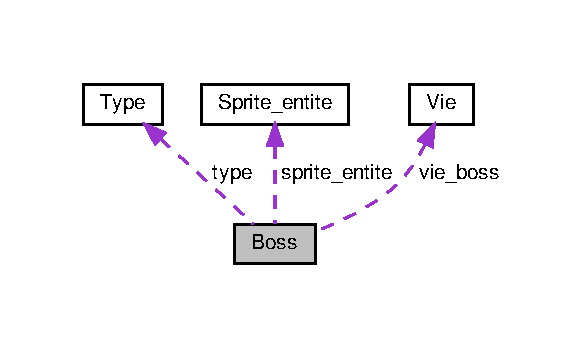
\includegraphics[width=281pt]{structBoss__coll__graph}
\end{center}
\end{figure}
\subsection*{Data Fields}
\begin{DoxyCompactItemize}
\item 
\mbox{\Hypertarget{structBoss_a26df6e28cbdbc1cb5111e65f61b15e01}\label{structBoss_a26df6e28cbdbc1cb5111e65f61b15e01}} 
S\+D\+L\+\_\+\+Rect {\bfseries pos\+Max}
\item 
\mbox{\Hypertarget{structBoss_a6c6ba05e3456c37d05068dc544196708}\label{structBoss_a6c6ba05e3456c37d05068dc544196708}} 
S\+D\+L\+\_\+\+Rect {\bfseries pos\+Min}
\item 
\mbox{\Hypertarget{structBoss_a81428638da280c4577f023f973efa10e}\label{structBoss_a81428638da280c4577f023f973efa10e}} 
S\+D\+L\+\_\+\+Rect {\bfseries position}
\item 
\mbox{\Hypertarget{structBoss_af5f26c9500124e1b4e48bb9ce85621e9}\label{structBoss_af5f26c9500124e1b4e48bb9ce85621e9}} 
\hyperlink{structSprite__entite}{sprite\+\_\+entite} {\bfseries sprite\+\_\+entite}
\item 
\mbox{\Hypertarget{structBoss_a7d48cc08f4061c623f689bde0c826393}\label{structBoss_a7d48cc08f4061c623f689bde0c826393}} 
\hyperlink{structstate__entite}{state\+\_\+entite} {\bfseries state\+\_\+entite}
\item 
\mbox{\Hypertarget{structBoss_a370a0d1e022a39f54ee7f5ef6f880f86}\label{structBoss_a370a0d1e022a39f54ee7f5ef6f880f86}} 
int {\bfseries direction\+\_\+entite}
\item 
\mbox{\Hypertarget{structBoss_ab1b35c434f7a9a21712d1f4cfde34bcc}\label{structBoss_ab1b35c434f7a9a21712d1f4cfde34bcc}} 
\hyperlink{structVie}{vie} {\bfseries vie\+\_\+boss}
\item 
\mbox{\Hypertarget{structBoss_a60c3ad92fac6b0daf8e1def7cd61bf1f}\label{structBoss_a60c3ad92fac6b0daf8e1def7cd61bf1f}} 
type {\bfseries type}
\item 
\mbox{\Hypertarget{structBoss_adcc7d6706d1cfdf76466d1311cd15160}\label{structBoss_adcc7d6706d1cfdf76466d1311cd15160}} 
int {\bfseries vitesse}
\item 
\mbox{\Hypertarget{structBoss_a6220f90cd65e9c2c451e3a49ad3b76d2}\label{structBoss_a6220f90cd65e9c2c451e3a49ad3b76d2}} 
S\+D\+L\+\_\+\+Surface $\ast$ {\bfseries health\+\_\+full}
\item 
\mbox{\Hypertarget{structBoss_aade0212329d8db9faddb70d1f1699c66}\label{structBoss_aade0212329d8db9faddb70d1f1699c66}} 
S\+D\+L\+\_\+\+Surface $\ast$ {\bfseries health\+\_\+empty}
\item 
\mbox{\Hypertarget{structBoss_a5e267a56ed1bb879225eda32f0840709}\label{structBoss_a5e267a56ed1bb879225eda32f0840709}} 
S\+D\+L\+\_\+\+Surface $\ast$ {\bfseries health\+\_\+1}
\item 
\mbox{\Hypertarget{structBoss_a79ae6a499c2a1d4612c13647daeef0e6}\label{structBoss_a79ae6a499c2a1d4612c13647daeef0e6}} 
S\+D\+L\+\_\+\+Surface $\ast$ {\bfseries health\+\_\+2}
\item 
\mbox{\Hypertarget{structBoss_ac6a96200cdc211f117c3cc83b15b1150}\label{structBoss_ac6a96200cdc211f117c3cc83b15b1150}} 
S\+D\+L\+\_\+\+Surface $\ast$ {\bfseries health\+\_\+3}
\item 
\mbox{\Hypertarget{structBoss_ac589e0fccda69d672f8510adf3520e7e}\label{structBoss_ac589e0fccda69d672f8510adf3520e7e}} 
S\+D\+L\+\_\+\+Rect {\bfseries pos\+\_\+health}
\end{DoxyCompactItemize}


\subsection{Detailed Description}
the boss stuct 

The documentation for this struct was generated from the following file\+:\begin{DoxyCompactItemize}
\item 
entite\+\_\+secondaire.\+h\end{DoxyCompactItemize}

\hypertarget{structButton}{}\section{Button Struct Reference}
\label{structButton}\index{Button@{Button}}


For loading a button.  




{\ttfamily \#include $<$menu.\+h$>$}

\subsection*{Data Fields}
\begin{DoxyCompactItemize}
\item 
\mbox{\Hypertarget{structButton_a9b46ba5cac45b47ada9d1491ffff575d}\label{structButton_a9b46ba5cac45b47ada9d1491ffff575d}} 
S\+D\+L\+\_\+\+Surface $\ast$ {\bfseries image}
\item 
\mbox{\Hypertarget{structButton_a0343ba330902623017b8915e2d629a83}\label{structButton_a0343ba330902623017b8915e2d629a83}} 
S\+D\+L\+\_\+\+Rect {\bfseries position}
\end{DoxyCompactItemize}


\subsection{Detailed Description}
For loading a button. 

The documentation for this struct was generated from the following file\+:\begin{DoxyCompactItemize}
\item 
menu.\+h\end{DoxyCompactItemize}

\hypertarget{structcharacter}{}\section{character Struct Reference}
\label{structcharacter}\index{character@{character}}


for character choice  




{\ttfamily \#include $<$structs.\+h$>$}



\subsection{Detailed Description}
for character choice 

The documentation for this struct was generated from the following file\+:\begin{DoxyCompactItemize}
\item 
structs.\+h\end{DoxyCompactItemize}

\hypertarget{structChoice}{}\section{Choice Struct Reference}
\label{structChoice}\index{Choice@{Choice}}


To account for the choice.  




{\ttfamily \#include $<$menu.\+h$>$}



\subsection{Detailed Description}
To account for the choice. 

The documentation for this struct was generated from the following file\+:\begin{DoxyCompactItemize}
\item 
menu.\+h\end{DoxyCompactItemize}

\hypertarget{structchoice__button}{}\section{choice\+\_\+button Struct Reference}
\label{structchoice__button}\index{choice\+\_\+button@{choice\+\_\+button}}


To update buttons in the menu.  




{\ttfamily \#include $<$menu.\+h$>$}



\subsection{Detailed Description}
To update buttons in the menu. 

The documentation for this struct was generated from the following file\+:\begin{DoxyCompactItemize}
\item 
menu.\+h\end{DoxyCompactItemize}

\hypertarget{structDialogue}{}\section{Dialogue Struct Reference}
\label{structDialogue}\index{Dialogue@{Dialogue}}


To load the dialogue in the game.  




{\ttfamily \#include $<$hero.\+h$>$}



Collaboration diagram for Dialogue\+:\nopagebreak
\begin{figure}[H]
\begin{center}
\leavevmode
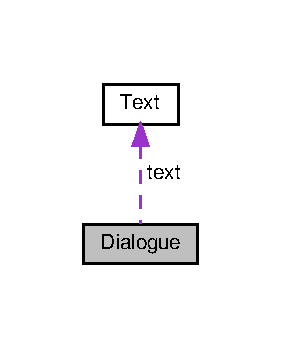
\includegraphics[width=135pt]{structDialogue__coll__graph}
\end{center}
\end{figure}
\subsection*{Data Fields}
\begin{DoxyCompactItemize}
\item 
\mbox{\Hypertarget{structDialogue_a468a4ed40fc86b7b9e8ad36b85af9ed9}\label{structDialogue_a468a4ed40fc86b7b9e8ad36b85af9ed9}} 
\hyperlink{structtext}{text} {\bfseries text}
\item 
\mbox{\Hypertarget{structDialogue_adeefc1c305f4c968d8f93d609d1300ce}\label{structDialogue_adeefc1c305f4c968d8f93d609d1300ce}} 
char {\bfseries script} \mbox{[}20\mbox{]}\mbox{[}40\mbox{]}
\item 
\mbox{\Hypertarget{structDialogue_a71983813bfe132b35f8faff9b78f0d16}\label{structDialogue_a71983813bfe132b35f8faff9b78f0d16}} 
S\+D\+L\+\_\+\+Surface $\ast$ {\bfseries dialogue\+\_\+box}
\item 
\mbox{\Hypertarget{structDialogue_a7c24d1a699a47a9fefda94cf300b1c37}\label{structDialogue_a7c24d1a699a47a9fefda94cf300b1c37}} 
S\+D\+L\+\_\+\+Surface $\ast$ {\bfseries hero\+\_\+dialogue}
\item 
\mbox{\Hypertarget{structDialogue_af71b90933f9885932ce341dc0e873697}\label{structDialogue_af71b90933f9885932ce341dc0e873697}} 
S\+D\+L\+\_\+\+Rect {\bfseries pos\+\_\+dialogue\+\_\+box}
\item 
\mbox{\Hypertarget{structDialogue_aa20be35dbfed8b7a4e47c4752db6490a}\label{structDialogue_aa20be35dbfed8b7a4e47c4752db6490a}} 
S\+D\+L\+\_\+\+Rect {\bfseries pos\+\_\+hero\+\_\+dialogue}
\item 
\mbox{\Hypertarget{structDialogue_abb24b97d5e978d5459abd474a2521940}\label{structDialogue_abb24b97d5e978d5459abd474a2521940}} 
int {\bfseries line}
\item 
\mbox{\Hypertarget{structDialogue_a843bd3e6ea34d7e9eb8b240629d4158b}\label{structDialogue_a843bd3e6ea34d7e9eb8b240629d4158b}} 
int {\bfseries talking}
\item 
\mbox{\Hypertarget{structDialogue_a813c5d98ac22180b91f7e48a3d0e9f46}\label{structDialogue_a813c5d98ac22180b91f7e48a3d0e9f46}} 
int {\bfseries first\+\_\+time}
\end{DoxyCompactItemize}


\subsection{Detailed Description}
To load the dialogue in the game. 

The documentation for this struct was generated from the following file\+:\begin{DoxyCompactItemize}
\item 
hero.\+h\end{DoxyCompactItemize}

\hypertarget{structDirection}{}\section{Direction Struct Reference}
\label{structDirection}\index{Direction@{Direction}}


Describe the hero direction.  




{\ttfamily \#include $<$hero.\+h$>$}



\subsection{Detailed Description}
Describe the hero direction. 

The documentation for this struct was generated from the following file\+:\begin{DoxyCompactItemize}
\item 
hero.\+h\end{DoxyCompactItemize}

\hypertarget{structenigme}{}\section{enigme Struct Reference}
\label{structenigme}\index{enigme@{enigme}}


struct for the enigma  




{\ttfamily \#include $<$enigme.\+h$>$}

\subsection*{Data Fields}
\begin{DoxyCompactItemize}
\item 
\mbox{\Hypertarget{structenigme_afef580eaca259227dac7bbae2d09f8f7}\label{structenigme_afef580eaca259227dac7bbae2d09f8f7}} 
S\+D\+L\+\_\+\+Surface $\ast$ {\bfseries background}
\item 
\mbox{\Hypertarget{structenigme_a10ee397636fe45d16379476fb990c58a}\label{structenigme_a10ee397636fe45d16379476fb990c58a}} 
S\+D\+L\+\_\+\+Surface $\ast$ {\bfseries bgansewr}
\item 
\mbox{\Hypertarget{structenigme_aebbf2d7046b5e0545f7b84fef6e98831}\label{structenigme_aebbf2d7046b5e0545f7b84fef6e98831}} 
S\+D\+L\+\_\+\+Surface $\ast$ {\bfseries bghover}
\item 
\mbox{\Hypertarget{structenigme_a917462fa7abd51385bfb39274d24c11f}\label{structenigme_a917462fa7abd51385bfb39274d24c11f}} 
S\+D\+L\+\_\+\+Surface $\ast$ {\bfseries Question}
\item 
\mbox{\Hypertarget{structenigme_ab3a0b156348a72483447216e90c28af0}\label{structenigme_ab3a0b156348a72483447216e90c28af0}} 
S\+D\+L\+\_\+\+Surface $\ast$ {\bfseries ansewr1}
\item 
\mbox{\Hypertarget{structenigme_a97c066a4114758708b5b4400f07de023}\label{structenigme_a97c066a4114758708b5b4400f07de023}} 
S\+D\+L\+\_\+\+Surface $\ast$ {\bfseries ansewr2}
\item 
\mbox{\Hypertarget{structenigme_a49754c0a7b2de36218e07574b0df6ea4}\label{structenigme_a49754c0a7b2de36218e07574b0df6ea4}} 
S\+D\+L\+\_\+\+Surface $\ast$ {\bfseries ansewr3}
\item 
\mbox{\Hypertarget{structenigme_a4eb7509adf07f09049e9a375d249bea6}\label{structenigme_a4eb7509adf07f09049e9a375d249bea6}} 
S\+D\+L\+\_\+\+Surface $\ast$ {\bfseries ansewr4}
\item 
\mbox{\Hypertarget{structenigme_ad4909b90c50cc4caf5d702e18f83e335}\label{structenigme_ad4909b90c50cc4caf5d702e18f83e335}} 
S\+D\+L\+\_\+\+Surface $\ast$ {\bfseries Yes}
\item 
\mbox{\Hypertarget{structenigme_a630ac6f3949179ec340c9e71ad53faee}\label{structenigme_a630ac6f3949179ec340c9e71ad53faee}} 
S\+D\+L\+\_\+\+Surface $\ast$ {\bfseries No}
\item 
\mbox{\Hypertarget{structenigme_a38e749d7ae027b8a4b487a49b49fe671}\label{structenigme_a38e749d7ae027b8a4b487a49b49fe671}} 
S\+D\+L\+\_\+\+Surface $\ast$ {\bfseries Final}
\item 
\mbox{\Hypertarget{structenigme_ae0dd357e0952647ab0de64abc803b660}\label{structenigme_ae0dd357e0952647ab0de64abc803b660}} 
S\+D\+L\+\_\+\+Rect {\bfseries position\+Background}
\item 
\mbox{\Hypertarget{structenigme_abd09b99260062e8b2f5ec41c9eedbfae}\label{structenigme_abd09b99260062e8b2f5ec41c9eedbfae}} 
S\+D\+L\+\_\+\+Rect {\bfseries position\+Ansewr1}
\item 
\mbox{\Hypertarget{structenigme_a64fefb6cab2baaee1c0e54d51f4b5486}\label{structenigme_a64fefb6cab2baaee1c0e54d51f4b5486}} 
S\+D\+L\+\_\+\+Rect {\bfseries position\+Ansewr2}
\item 
\mbox{\Hypertarget{structenigme_aba195f6df5f2e975e2bb19983f2ae542}\label{structenigme_aba195f6df5f2e975e2bb19983f2ae542}} 
S\+D\+L\+\_\+\+Rect {\bfseries position\+Ansewr3}
\item 
\mbox{\Hypertarget{structenigme_a5b5c3043e61541f4c63c1bc55651ca51}\label{structenigme_a5b5c3043e61541f4c63c1bc55651ca51}} 
S\+D\+L\+\_\+\+Rect {\bfseries position\+Ansewr4}
\item 
\mbox{\Hypertarget{structenigme_ae10e2d3b647b0728eba96dcbc3098619}\label{structenigme_ae10e2d3b647b0728eba96dcbc3098619}} 
S\+D\+L\+\_\+\+Rect {\bfseries positionQ}
\item 
\mbox{\Hypertarget{structenigme_acbf34a299f6a43366abb738df85c282d}\label{structenigme_acbf34a299f6a43366abb738df85c282d}} 
S\+D\+L\+\_\+\+Rect {\bfseries positionhover}
\item 
\mbox{\Hypertarget{structenigme_a53787af725dae2956717fa2eba7ca6a9}\label{structenigme_a53787af725dae2956717fa2eba7ca6a9}} 
S\+D\+L\+\_\+\+Rect {\bfseries position\+Final}
\item 
\mbox{\Hypertarget{structenigme_af7467a612a16fb5cdd6707dd80e52269}\label{structenigme_af7467a612a16fb5cdd6707dd80e52269}} 
int {\bfseries rangR}
\item 
\mbox{\Hypertarget{structenigme_aecd303e40283cd9e1480aa937104266a}\label{structenigme_aecd303e40283cd9e1480aa937104266a}} 
int {\bfseries resolution}
\end{DoxyCompactItemize}


\subsection{Detailed Description}
struct for the enigma 

The documentation for this struct was generated from the following file\+:\begin{DoxyCompactItemize}
\item 
enigme.\+h\end{DoxyCompactItemize}

\hypertarget{structEntite}{}\section{Entite Struct Reference}
\label{structEntite}\index{Entite@{Entite}}


General entity struct.  




{\ttfamily \#include $<$entite\+\_\+secondaire.\+h$>$}



Collaboration diagram for Entite\+:
\nopagebreak
\begin{figure}[H]
\begin{center}
\leavevmode
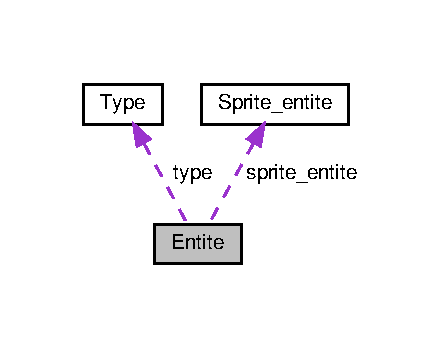
\includegraphics[width=212pt]{structEntite__coll__graph}
\end{center}
\end{figure}
\subsection*{Data Fields}
\begin{DoxyCompactItemize}
\item 
\mbox{\Hypertarget{structEntite_a9a50f732529d9d4fadb3f2a84f7c100e}\label{structEntite_a9a50f732529d9d4fadb3f2a84f7c100e}} 
S\+D\+L\+\_\+\+Rect {\bfseries pos\+Max}
\item 
\mbox{\Hypertarget{structEntite_a423bb0869194e380e2eeed768abc25e7}\label{structEntite_a423bb0869194e380e2eeed768abc25e7}} 
S\+D\+L\+\_\+\+Rect {\bfseries pos\+Min}
\item 
\mbox{\Hypertarget{structEntite_ab7d2d161df4c728b71096310110fc42f}\label{structEntite_ab7d2d161df4c728b71096310110fc42f}} 
S\+D\+L\+\_\+\+Rect {\bfseries position}
\item 
\mbox{\Hypertarget{structEntite_a02737936435247b355900e31b6f25a6a}\label{structEntite_a02737936435247b355900e31b6f25a6a}} 
\hyperlink{structSprite__entite}{sprite\+\_\+entite} {\bfseries sprite\+\_\+entite}
\item 
\mbox{\Hypertarget{structEntite_a1427b445875a07252153acfae59d5e29}\label{structEntite_a1427b445875a07252153acfae59d5e29}} 
\hyperlink{structstate__entite}{state\+\_\+entite} {\bfseries state\+\_\+entite}
\item 
\mbox{\Hypertarget{structEntite_aaf0a2ea54f84354fa8d31df7b20456d8}\label{structEntite_aaf0a2ea54f84354fa8d31df7b20456d8}} 
int {\bfseries direction\+\_\+entite}
\item 
\mbox{\Hypertarget{structEntite_a7a72d6d6556d3e526e3a2a5c197b17cd}\label{structEntite_a7a72d6d6556d3e526e3a2a5c197b17cd}} 
type {\bfseries type}
\item 
\mbox{\Hypertarget{structEntite_a7b94da47ebaa582ad59e0b692a04b8fa}\label{structEntite_a7b94da47ebaa582ad59e0b692a04b8fa}} 
int {\bfseries vitesse}
\end{DoxyCompactItemize}


\subsection{Detailed Description}
General entity struct. 

The documentation for this struct was generated from the following file\+:\begin{DoxyCompactItemize}
\item 
entite\+\_\+secondaire.\+h\end{DoxyCompactItemize}

\hypertarget{structetat}{}\section{etat Struct Reference}
\label{structetat}\index{etat@{etat}}


for the game state  




{\ttfamily \#include $<$structs.\+h$>$}



\subsection{Detailed Description}
for the game state 

The documentation for this struct was generated from the following file\+:\begin{DoxyCompactItemize}
\item 
structs.\+h\end{DoxyCompactItemize}

\hypertarget{structheart}{}\section{heart Struct Reference}
\label{structheart}\index{heart@{heart}}


the heart you collect  




{\ttfamily \#include $<$entite\+\_\+secondaire.\+h$>$}



\subsection{Detailed Description}
the heart you collect 

The documentation for this struct was generated from the following file\+:\begin{DoxyCompactItemize}
\item 
entite\+\_\+secondaire.\+h\end{DoxyCompactItemize}

\hypertarget{structHeart}{}\section{Heart Struct Reference}
\label{structHeart}\index{Heart@{Heart}}
\subsection*{Data Fields}
\begin{DoxyCompactItemize}
\item 
\mbox{\Hypertarget{structHeart_a9a0f6ed60e258415e83bdb5a3118e151}\label{structHeart_a9a0f6ed60e258415e83bdb5a3118e151}} 
S\+D\+L\+\_\+\+Surface $\ast$ {\bfseries image}
\item 
\mbox{\Hypertarget{structHeart_ac4d13d2d7a77af3cd8822b18d35168a2}\label{structHeart_ac4d13d2d7a77af3cd8822b18d35168a2}} 
S\+D\+L\+\_\+\+Rect {\bfseries position}
\item 
\mbox{\Hypertarget{structHeart_a9a9aa1322dd7d19c8fae369723ebd865}\label{structHeart_a9a9aa1322dd7d19c8fae369723ebd865}} 
Mix\+\_\+\+Chunk $\ast$ {\bfseries click}
\item 
\mbox{\Hypertarget{structHeart_a58e54316de92b359afa6c753b689fbdc}\label{structHeart_a58e54316de92b359afa6c753b689fbdc}} 
S\+D\+L\+\_\+\+Rect {\bfseries pos\+\_\+init}
\end{DoxyCompactItemize}


The documentation for this struct was generated from the following file\+:\begin{DoxyCompactItemize}
\item 
entite\+\_\+secondaire.\+h\end{DoxyCompactItemize}

\hypertarget{structHero}{}\section{Hero Struct Reference}
\label{structHero}\index{Hero@{Hero}}


anything used by the main character  




{\ttfamily \#include $<$hero.\+h$>$}



Collaboration diagram for Hero\+:
\nopagebreak
\begin{figure}[H]
\begin{center}
\leavevmode
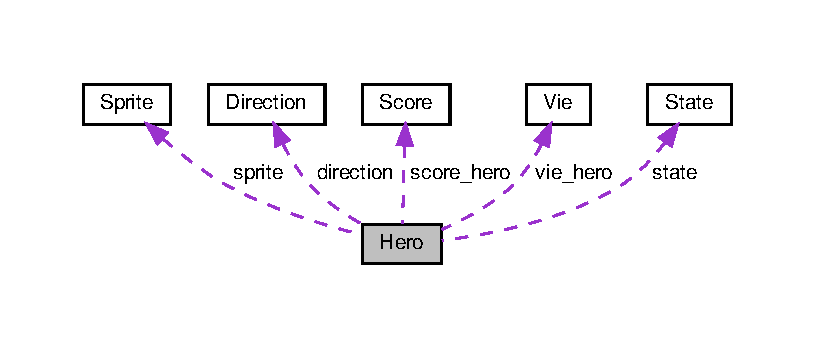
\includegraphics[width=350pt]{structHero__coll__graph}
\end{center}
\end{figure}
\subsection*{Data Fields}
\begin{DoxyCompactItemize}
\item 
\mbox{\Hypertarget{structHero_abc9595e897232ee4cf912e0e2c36bf28}\label{structHero_abc9595e897232ee4cf912e0e2c36bf28}} 
S\+D\+L\+\_\+\+Rect {\bfseries position}
\item 
\mbox{\Hypertarget{structHero_a1f280d48754ed952298adf26a5f10c16}\label{structHero_a1f280d48754ed952298adf26a5f10c16}} 
\hyperlink{structSprite}{sprite} {\bfseries sprite}
\item 
\mbox{\Hypertarget{structHero_af2abe9c576d42b2dffb36f2dc332d680}\label{structHero_af2abe9c576d42b2dffb36f2dc332d680}} 
state {\bfseries state}
\item 
\mbox{\Hypertarget{structHero_aa111c732e587bf2bee3f58c4e3c7dba3}\label{structHero_aa111c732e587bf2bee3f58c4e3c7dba3}} 
int {\bfseries collision\+\_\+\+UP}
\item 
\mbox{\Hypertarget{structHero_ab77a2aee8cecfbe25f95542179cfba65}\label{structHero_ab77a2aee8cecfbe25f95542179cfba65}} 
int {\bfseries collision\+\_\+\+D\+O\+WN}
\item 
\mbox{\Hypertarget{structHero_af8d0fe553ca11082004c8fdab84780e4}\label{structHero_af8d0fe553ca11082004c8fdab84780e4}} 
int {\bfseries collision\+\_\+\+R\+I\+G\+HT}
\item 
\mbox{\Hypertarget{structHero_af7f5cea2cc6cc1a0a71c6406f5cb7eb0}\label{structHero_af7f5cea2cc6cc1a0a71c6406f5cb7eb0}} 
int {\bfseries collision\+\_\+\+L\+E\+FT}
\item 
\mbox{\Hypertarget{structHero_ad0cda8d82f4351c33ac99403fad1ca52}\label{structHero_ad0cda8d82f4351c33ac99403fad1ca52}} 
int {\bfseries collision\+\_\+\+D\+O\+W\+N\+\_\+\+P\+L\+AT}
\item 
\mbox{\Hypertarget{structHero_a058a4906f1625db7ce2c1abcc4eca639}\label{structHero_a058a4906f1625db7ce2c1abcc4eca639}} 
int {\bfseries current\+\_\+ground\+\_\+position}
\item 
\mbox{\Hypertarget{structHero_ac32ab152105eb5cda88226f29ee03daf}\label{structHero_ac32ab152105eb5cda88226f29ee03daf}} 
direction {\bfseries direction}
\item 
\mbox{\Hypertarget{structHero_ab523a8e24b06bab0cbc17cd744f772aa}\label{structHero_ab523a8e24b06bab0cbc17cd744f772aa}} 
\hyperlink{structVie}{vie} {\bfseries vie\+\_\+hero}
\item 
\mbox{\Hypertarget{structHero_af3b8a739baa871df683f7ce374fae8d3}\label{structHero_af3b8a739baa871df683f7ce374fae8d3}} 
\hyperlink{structScore}{score} {\bfseries score\+\_\+hero}
\end{DoxyCompactItemize}


\subsection{Detailed Description}
anything used by the main character 

The documentation for this struct was generated from the following file\+:\begin{DoxyCompactItemize}
\item 
hero.\+h\end{DoxyCompactItemize}

\hypertarget{structHeure}{}\section{Heure Struct Reference}
\label{structHeure}\index{Heure@{Heure}}
\subsection*{Data Fields}
\begin{DoxyCompactItemize}
\item 
\mbox{\Hypertarget{structHeure_ae49d0f4a02685669f717f1617b564a57}\label{structHeure_ae49d0f4a02685669f717f1617b564a57}} 
int {\bfseries heures}
\item 
\mbox{\Hypertarget{structHeure_add82a2eaf354bbe3872ca4387f222295}\label{structHeure_add82a2eaf354bbe3872ca4387f222295}} 
int {\bfseries minutes}
\item 
\mbox{\Hypertarget{structHeure_ad0d5caf9f781db4389b8514d5ecffbd3}\label{structHeure_ad0d5caf9f781db4389b8514d5ecffbd3}} 
int {\bfseries secondes}
\end{DoxyCompactItemize}


The documentation for this struct was generated from the following file\+:\begin{DoxyCompactItemize}
\item 
background.\+h\end{DoxyCompactItemize}

\hypertarget{structheure}{}\section{heure Struct Reference}
\label{structheure}\index{heure@{heure}}


for time  




{\ttfamily \#include $<$background.\+h$>$}



\subsection{Detailed Description}
for time 

The documentation for this struct was generated from the following file\+:\begin{DoxyCompactItemize}
\item 
background.\+h\end{DoxyCompactItemize}

\hypertarget{structMat}{}\section{Mat Struct Reference}
\label{structMat}\index{Mat@{Mat}}
\subsection*{Data Fields}
\begin{DoxyCompactItemize}
\item 
\mbox{\Hypertarget{structMat_a01bad0c62ccd5aadb041c2f55a92d57e}\label{structMat_a01bad0c62ccd5aadb041c2f55a92d57e}} 
S\+D\+L\+\_\+\+Surface $\ast$ {\bfseries image}
\item 
\mbox{\Hypertarget{structMat_a739ffbb7e00b7331964550bece4ece1e}\label{structMat_a739ffbb7e00b7331964550bece4ece1e}} 
S\+D\+L\+\_\+\+Rect {\bfseries position}
\item 
\mbox{\Hypertarget{structMat_a280f9d2011149d891d2e5f9c5672c78d}\label{structMat_a280f9d2011149d891d2e5f9c5672c78d}} 
S\+D\+L\+\_\+\+Rect {\bfseries position\+\_\+init}
\end{DoxyCompactItemize}


The documentation for this struct was generated from the following file\+:\begin{DoxyCompactItemize}
\item 
entite\+\_\+secondaire.\+h\end{DoxyCompactItemize}

\hypertarget{structMatchstick}{}\section{Matchstick Struct Reference}
\label{structMatchstick}\index{Matchstick@{Matchstick}}


To load the match image.  




{\ttfamily \#include $<$matchsticks.\+h$>$}

\subsection*{Data Fields}
\begin{DoxyCompactItemize}
\item 
\mbox{\Hypertarget{structMatchstick_abf32429755f84e6d66e91498255c618f}\label{structMatchstick_abf32429755f84e6d66e91498255c618f}} 
S\+D\+L\+\_\+\+Surface $\ast$ {\bfseries Matchstick}
\item 
\mbox{\Hypertarget{structMatchstick_a94b7cf5a0090423782617da879344d2b}\label{structMatchstick_a94b7cf5a0090423782617da879344d2b}} 
S\+D\+L\+\_\+\+Rect {\bfseries position\+Matchstick}
\item 
\mbox{\Hypertarget{structMatchstick_a7b99dba66cb2d9fabe1c74ab96c677b2}\label{structMatchstick_a7b99dba66cb2d9fabe1c74ab96c677b2}} 
int {\bfseries Match\+Count}
\end{DoxyCompactItemize}


\subsection{Detailed Description}
To load the match image. 

The documentation for this struct was generated from the following file\+:\begin{DoxyCompactItemize}
\item 
matchsticks.\+h\end{DoxyCompactItemize}

\hypertarget{structMinimap}{}\section{Minimap Struct Reference}
\label{structMinimap}\index{Minimap@{Minimap}}
\subsection*{Data Fields}
\begin{DoxyCompactItemize}
\item 
\mbox{\Hypertarget{structMinimap_ae1792d7a5459227ec30b7c1e84a586fc}\label{structMinimap_ae1792d7a5459227ec30b7c1e84a586fc}} 
S\+D\+L\+\_\+\+Surface $\ast$ {\bfseries image}
\item 
\mbox{\Hypertarget{structMinimap_a8ed3ce99bcaf1dfc85548642abe7b8c7}\label{structMinimap_a8ed3ce99bcaf1dfc85548642abe7b8c7}} 
S\+D\+L\+\_\+\+Surface $\ast$ {\bfseries hero}
\item 
\mbox{\Hypertarget{structMinimap_a36d34abc386e8bae78f7adf4c43e6f0d}\label{structMinimap_a36d34abc386e8bae78f7adf4c43e6f0d}} 
S\+D\+L\+\_\+\+Rect {\bfseries pos\+\_\+image}
\item 
\mbox{\Hypertarget{structMinimap_a6b55710065e1c7b804d48fa8087f8824}\label{structMinimap_a6b55710065e1c7b804d48fa8087f8824}} 
S\+D\+L\+\_\+\+Rect {\bfseries pos\+\_\+hero}
\end{DoxyCompactItemize}


The documentation for this struct was generated from the following file\+:\begin{DoxyCompactItemize}
\item 
background.\+h\end{DoxyCompactItemize}

\hypertarget{structminimap}{}\section{minimap Struct Reference}
\label{structminimap}\index{minimap@{minimap}}


for the minimap  




{\ttfamily \#include $<$background.\+h$>$}



\subsection{Detailed Description}
for the minimap 

The documentation for this struct was generated from the following file\+:\begin{DoxyCompactItemize}
\item 
background.\+h\end{DoxyCompactItemize}

\hypertarget{structparameter}{}\section{parameter Struct Reference}
\label{structparameter}\index{parameter@{parameter}}


for the game settings  




{\ttfamily \#include $<$structs.\+h$>$}



\subsection{Detailed Description}
for the game settings 

The documentation for this struct was generated from the following file\+:\begin{DoxyCompactItemize}
\item 
structs.\+h\end{DoxyCompactItemize}

\hypertarget{structParameter}{}\section{Parameter Struct Reference}
\label{structParameter}\index{Parameter@{Parameter}}
\subsection*{Data Fields}
\begin{DoxyCompactItemize}
\item 
\mbox{\Hypertarget{structParameter_aa7dbc1acec97da51a2a4e6346d890b4f}\label{structParameter_aa7dbc1acec97da51a2a4e6346d890b4f}} 
Mix\+\_\+\+Music $\ast$ {\bfseries music}
\item 
\mbox{\Hypertarget{structParameter_a48918a3e4a9514cffb9b59dd85c511cd}\label{structParameter_a48918a3e4a9514cffb9b59dd85c511cd}} 
Mix\+\_\+\+Chunk $\ast$ {\bfseries click}
\item 
\mbox{\Hypertarget{structParameter_ae04ba3c3bdee5642a2d591e256823d3e}\label{structParameter_ae04ba3c3bdee5642a2d591e256823d3e}} 
Mix\+\_\+\+Chunk $\ast$ {\bfseries keyboard\+\_\+click}
\item 
\mbox{\Hypertarget{structParameter_a8041ac8b22ef7c28648ae0d0ebc61698}\label{structParameter_a8041ac8b22ef7c28648ae0d0ebc61698}} 
int {\bfseries volume}
\item 
\mbox{\Hypertarget{structParameter_a51bd6883effe03e02ff0f262b47c724a}\label{structParameter_a51bd6883effe03e02ff0f262b47c724a}} 
int {\bfseries fullscreen}
\item 
\mbox{\Hypertarget{structParameter_aacb7d19d4e42e7880c3606629b08bfa5}\label{structParameter_aacb7d19d4e42e7880c3606629b08bfa5}} 
int {\bfseries mute}
\end{DoxyCompactItemize}


The documentation for this struct was generated from the following file\+:\begin{DoxyCompactItemize}
\item 
structs.\+h\end{DoxyCompactItemize}

\hypertarget{structPlatforme}{}\section{Platforme Struct Reference}
\label{structPlatforme}\index{Platforme@{Platforme}}
\subsection*{Data Fields}
\begin{DoxyCompactItemize}
\item 
\mbox{\Hypertarget{structPlatforme_a1fededad065363039bf9a5969a52819e}\label{structPlatforme_a1fededad065363039bf9a5969a52819e}} 
S\+D\+L\+\_\+\+Surface $\ast$ {\bfseries image}
\item 
\mbox{\Hypertarget{structPlatforme_af2c9e89d1a8db9aecbfac2ca8a248407}\label{structPlatforme_af2c9e89d1a8db9aecbfac2ca8a248407}} 
S\+D\+L\+\_\+\+Rect {\bfseries position}
\item 
\mbox{\Hypertarget{structPlatforme_a7a50d184a18f9572aee7d2ff3e4ec6ca}\label{structPlatforme_a7a50d184a18f9572aee7d2ff3e4ec6ca}} 
S\+D\+L\+\_\+\+Rect {\bfseries pos\+\_\+init}
\item 
\mbox{\Hypertarget{structPlatforme_a254e58d9278e4a6ec01de25009e86d1b}\label{structPlatforme_a254e58d9278e4a6ec01de25009e86d1b}} 
int {\bfseries interval}
\item 
\mbox{\Hypertarget{structPlatforme_a7ad73bffce8c77d18d617513f5fc90a9}\label{structPlatforme_a7ad73bffce8c77d18d617513f5fc90a9}} 
int {\bfseries sens}
\end{DoxyCompactItemize}


The documentation for this struct was generated from the following file\+:\begin{DoxyCompactItemize}
\item 
background.\+h\end{DoxyCompactItemize}

\hypertarget{structplatforme}{}\section{platforme Struct Reference}
\label{structplatforme}\index{platforme@{platforme}}


for platforme  




{\ttfamily \#include $<$background.\+h$>$}



\subsection{Detailed Description}
for platforme 

The documentation for this struct was generated from the following file\+:\begin{DoxyCompactItemize}
\item 
background.\+h\end{DoxyCompactItemize}

\hypertarget{structPortal}{}\section{Portal Struct Reference}
\label{structPortal}\index{Portal@{Portal}}


for the portal  




{\ttfamily \#include $<$background.\+h$>$}

\subsection*{Data Fields}
\begin{DoxyCompactItemize}
\item 
\mbox{\Hypertarget{structPortal_a77ddecc0900365f5ca013351d32fc9ee}\label{structPortal_a77ddecc0900365f5ca013351d32fc9ee}} 
S\+D\+L\+\_\+\+Surface $\ast$ {\bfseries still} \mbox{[}4\mbox{]}
\item 
\mbox{\Hypertarget{structPortal_ab57554378c76f1c1d35022280aa250a1}\label{structPortal_ab57554378c76f1c1d35022280aa250a1}} 
S\+D\+L\+\_\+\+Surface $\ast$ {\bfseries enter} \mbox{[}15\mbox{]}
\item 
\mbox{\Hypertarget{structPortal_a241b257fc05abc880eca67c0db1e52ea}\label{structPortal_a241b257fc05abc880eca67c0db1e52ea}} 
S\+D\+L\+\_\+\+Rect {\bfseries pos\+\_\+enter}
\item 
\mbox{\Hypertarget{structPortal_a3cfcaf2bd0b3f229a073b7e7f1f2dc08}\label{structPortal_a3cfcaf2bd0b3f229a073b7e7f1f2dc08}} 
S\+D\+L\+\_\+\+Rect {\bfseries pos\+\_\+still}
\item 
\mbox{\Hypertarget{structPortal_ab3181fde5c8374c3c461f824b948221f}\label{structPortal_ab3181fde5c8374c3c461f824b948221f}} 
int {\bfseries frame\+\_\+still}
\item 
\mbox{\Hypertarget{structPortal_a5aab8cbcf440db0c100ab2e8fb267bf8}\label{structPortal_a5aab8cbcf440db0c100ab2e8fb267bf8}} 
int {\bfseries frame\+\_\+enter}
\end{DoxyCompactItemize}


\subsection{Detailed Description}
for the portal 

The documentation for this struct was generated from the following file\+:\begin{DoxyCompactItemize}
\item 
background.\+h\end{DoxyCompactItemize}

\hypertarget{structpower__up}{}\section{power\+\_\+up Struct Reference}
\label{structpower__up}\index{power\+\_\+up@{power\+\_\+up}}


the power up you collect  




{\ttfamily \#include $<$entite\+\_\+secondaire.\+h$>$}



\subsection{Detailed Description}
the power up you collect 

The documentation for this struct was generated from the following file\+:\begin{DoxyCompactItemize}
\item 
entite\+\_\+secondaire.\+h\end{DoxyCompactItemize}

\hypertarget{structPower__up}{}\section{Power\+\_\+up Struct Reference}
\label{structPower__up}\index{Power\+\_\+up@{Power\+\_\+up}}


Collaboration diagram for Power\+\_\+up\+:
\nopagebreak
\begin{figure}[H]
\begin{center}
\leavevmode
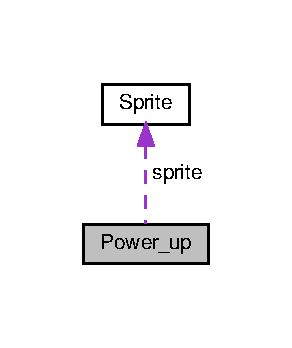
\includegraphics[width=140pt]{structPower__up__coll__graph}
\end{center}
\end{figure}
\subsection*{Data Fields}
\begin{DoxyCompactItemize}
\item 
\mbox{\Hypertarget{structPower__up_a76e1d05c017a2491cda4ac0d3014f0eb}\label{structPower__up_a76e1d05c017a2491cda4ac0d3014f0eb}} 
\hyperlink{structSprite}{sprite} {\bfseries sprite}
\item 
\mbox{\Hypertarget{structPower__up_a7369bc0bc57931b751b8889641819c4d}\label{structPower__up_a7369bc0bc57931b751b8889641819c4d}} 
S\+D\+L\+\_\+\+Rect {\bfseries position}
\item 
\mbox{\Hypertarget{structPower__up_ab062d39a523db0b01fd450575852b62b}\label{structPower__up_ab062d39a523db0b01fd450575852b62b}} 
Mix\+\_\+\+Chunk $\ast$ {\bfseries click}
\item 
\mbox{\Hypertarget{structPower__up_a928fc674bab68a3f650283e606ef16f2}\label{structPower__up_a928fc674bab68a3f650283e606ef16f2}} 
S\+D\+L\+\_\+\+Rect {\bfseries pos\+\_\+init}
\end{DoxyCompactItemize}


The documentation for this struct was generated from the following file\+:\begin{DoxyCompactItemize}
\item 
entite\+\_\+secondaire.\+h\end{DoxyCompactItemize}

\hypertarget{structScore}{}\section{Score Struct Reference}
\label{structScore}\index{Score@{Score}}


For score updating.  




{\ttfamily \#include $<$hero.\+h$>$}

\subsection*{Data Fields}
\begin{DoxyCompactItemize}
\item 
\mbox{\Hypertarget{structScore_ad9bae0529c9c744abdd0b1860b9731d2}\label{structScore_ad9bae0529c9c744abdd0b1860b9731d2}} 
S\+D\+L\+\_\+\+Surface $\ast$ {\bfseries texte\+\_\+score}
\item 
\mbox{\Hypertarget{structScore_ac5b7d95ca27a0c9527b1a3897c4a19d6}\label{structScore_ac5b7d95ca27a0c9527b1a3897c4a19d6}} 
S\+D\+L\+\_\+\+Rect {\bfseries position\+\_\+texte}
\item 
\mbox{\Hypertarget{structScore_a1d2d12c67fabfeb656b6660995d3d856}\label{structScore_a1d2d12c67fabfeb656b6660995d3d856}} 
T\+T\+F\+\_\+\+Font $\ast$ {\bfseries score\+\_\+font}
\item 
\mbox{\Hypertarget{structScore_a35b649d464a12207405d63b52a4afa58}\label{structScore_a35b649d464a12207405d63b52a4afa58}} 
S\+D\+L\+\_\+\+Color {\bfseries couleur\+Noire}
\item 
\mbox{\Hypertarget{structScore_a9188e7325c612cb5ece7a0f6c818089a}\label{structScore_a9188e7325c612cb5ece7a0f6c818089a}} 
int {\bfseries valeur\+\_\+score}
\end{DoxyCompactItemize}


\subsection{Detailed Description}
For score updating. 

The documentation for this struct was generated from the following file\+:\begin{DoxyCompactItemize}
\item 
hero.\+h\end{DoxyCompactItemize}

\hypertarget{structSprite}{}\section{Sprite Struct Reference}
\label{structSprite}\index{Sprite@{Sprite}}


to load and update the sprite  




{\ttfamily \#include $<$hero.\+h$>$}

\subsection*{Data Fields}
\begin{DoxyCompactItemize}
\item 
\mbox{\Hypertarget{structSprite_a80402c358e003c422aa75bec2b6d0099}\label{structSprite_a80402c358e003c422aa75bec2b6d0099}} 
S\+D\+L\+\_\+\+Surface $\ast$ {\bfseries image}
\item 
\mbox{\Hypertarget{structSprite_a3dab174a504c158e143e41960b7354f6}\label{structSprite_a3dab174a504c158e143e41960b7354f6}} 
S\+D\+L\+\_\+\+Rect {\bfseries frame}
\item 
\mbox{\Hypertarget{structSprite_a17956b3b5b551706a5aedde0bd06a234}\label{structSprite_a17956b3b5b551706a5aedde0bd06a234}} 
int {\bfseries curframe}
\item 
\mbox{\Hypertarget{structSprite_a0bbc4bad956af279f94539d476d9b9d2}\label{structSprite_a0bbc4bad956af279f94539d476d9b9d2}} 
int {\bfseries maxframe}
\end{DoxyCompactItemize}


\subsection{Detailed Description}
to load and update the sprite 

The documentation for this struct was generated from the following file\+:\begin{DoxyCompactItemize}
\item 
hero.\+h\end{DoxyCompactItemize}

\hypertarget{structSprite__entite}{}\section{Sprite\+\_\+entite Struct Reference}
\label{structSprite__entite}\index{Sprite\+\_\+entite@{Sprite\+\_\+entite}}


To load the enemy sprite.  




{\ttfamily \#include $<$entite\+\_\+secondaire.\+h$>$}

\subsection*{Data Fields}
\begin{DoxyCompactItemize}
\item 
\mbox{\Hypertarget{structSprite__entite_aa8dec7395027cdfa3b8143c4f02b7764}\label{structSprite__entite_aa8dec7395027cdfa3b8143c4f02b7764}} 
S\+D\+L\+\_\+\+Surface $\ast$ {\bfseries image}
\item 
\mbox{\Hypertarget{structSprite__entite_a8aa8da5e0b1bc226ebbab21e7ff299de}\label{structSprite__entite_a8aa8da5e0b1bc226ebbab21e7ff299de}} 
S\+D\+L\+\_\+\+Rect {\bfseries frame}
\item 
\mbox{\Hypertarget{structSprite__entite_ae7b29752e80665e4e7bd39d1c98aede3}\label{structSprite__entite_ae7b29752e80665e4e7bd39d1c98aede3}} 
int {\bfseries curframe}
\item 
\mbox{\Hypertarget{structSprite__entite_a4971a024d3c9f9695de89f11bc64cb73}\label{structSprite__entite_a4971a024d3c9f9695de89f11bc64cb73}} 
int {\bfseries maxframe}
\end{DoxyCompactItemize}


\subsection{Detailed Description}
To load the enemy sprite. 

The documentation for this struct was generated from the following file\+:\begin{DoxyCompactItemize}
\item 
entite\+\_\+secondaire.\+h\end{DoxyCompactItemize}

\hypertarget{structState}{}\section{State Struct Reference}
\label{structState}\index{State@{State}}


Describe the hero state.  




{\ttfamily \#include $<$hero.\+h$>$}



\subsection{Detailed Description}
Describe the hero state. 

The documentation for this struct was generated from the following file\+:\begin{DoxyCompactItemize}
\item 
hero.\+h\end{DoxyCompactItemize}

\hypertarget{structstate__entite}{}\section{state\+\_\+entite Struct Reference}
\label{structstate__entite}\index{state\+\_\+entite@{state\+\_\+entite}}


describes the enemy state  




{\ttfamily \#include $<$entite\+\_\+secondaire.\+h$>$}



\subsection{Detailed Description}
describes the enemy state 

The documentation for this struct was generated from the following file\+:\begin{DoxyCompactItemize}
\item 
entite\+\_\+secondaire.\+h\end{DoxyCompactItemize}

\hypertarget{structtext}{}\section{text Struct Reference}
\label{structtext}\index{text@{text}}


for text  




{\ttfamily \#include $<$background.\+h$>$}



\subsection{Detailed Description}
for text 

The documentation for this struct was generated from the following file\+:\begin{DoxyCompactItemize}
\item 
background.\+h\end{DoxyCompactItemize}

\hypertarget{structText}{}\section{Text Struct Reference}
\label{structText}\index{Text@{Text}}
\subsection*{Data Fields}
\begin{DoxyCompactItemize}
\item 
\mbox{\Hypertarget{structText_aff9f844dbb049d64f616d143376b7d55}\label{structText_aff9f844dbb049d64f616d143376b7d55}} 
S\+D\+L\+\_\+\+Surface $\ast$ {\bfseries text}
\item 
\mbox{\Hypertarget{structText_a6bedd1f0e3a1422ae4533301a8fe0641}\label{structText_a6bedd1f0e3a1422ae4533301a8fe0641}} 
S\+D\+L\+\_\+\+Rect {\bfseries position}
\item 
\mbox{\Hypertarget{structText_ae23ac53acb57e760b91c81d8c4aec8c7}\label{structText_ae23ac53acb57e760b91c81d8c4aec8c7}} 
T\+T\+F\+\_\+\+Font $\ast$ {\bfseries font}
\item 
\mbox{\Hypertarget{structText_ab0f771bd18d8e968f7aaee4a4e26e385}\label{structText_ab0f771bd18d8e968f7aaee4a4e26e385}} 
S\+D\+L\+\_\+\+Color {\bfseries color}
\item 
\mbox{\Hypertarget{structText_aeeefa18b9d848a532e402065815d21b7}\label{structText_aeeefa18b9d848a532e402065815d21b7}} 
int {\bfseries size}
\end{DoxyCompactItemize}


The documentation for this struct was generated from the following file\+:\begin{DoxyCompactItemize}
\item 
background.\+h\end{DoxyCompactItemize}

\hypertarget{structText__enigme}{}\section{Text\+\_\+enigme Struct Reference}
\label{structText__enigme}\index{Text\+\_\+enigme@{Text\+\_\+enigme}}


for text generation in the enigma  




{\ttfamily \#include $<$matchsticks.\+h$>$}

\subsection*{Data Fields}
\begin{DoxyCompactItemize}
\item 
\mbox{\Hypertarget{structText__enigme_a8e53db4f6d572ee05a3a5394c0b39885}\label{structText__enigme_a8e53db4f6d572ee05a3a5394c0b39885}} 
S\+D\+L\+\_\+\+Surface $\ast$ {\bfseries text}
\item 
\mbox{\Hypertarget{structText__enigme_a1014666a5119f333087f45987558a380}\label{structText__enigme_a1014666a5119f333087f45987558a380}} 
S\+D\+L\+\_\+\+Rect {\bfseries position}
\item 
\mbox{\Hypertarget{structText__enigme_aa6db3ad23e6a0b80e973cfdd4f8c45a7}\label{structText__enigme_aa6db3ad23e6a0b80e973cfdd4f8c45a7}} 
T\+T\+F\+\_\+\+Font $\ast$ {\bfseries font}
\item 
\mbox{\Hypertarget{structText__enigme_a281b95feb122066eedf8fd62bf728070}\label{structText__enigme_a281b95feb122066eedf8fd62bf728070}} 
S\+D\+L\+\_\+\+Color {\bfseries color1}
\item 
\mbox{\Hypertarget{structText__enigme_a0134c22d777c58b8025445de627e5b16}\label{structText__enigme_a0134c22d777c58b8025445de627e5b16}} 
S\+D\+L\+\_\+\+Color {\bfseries color2}
\item 
\mbox{\Hypertarget{structText__enigme_a716eb1e88e41e1679ee0b94c89f2b861}\label{structText__enigme_a716eb1e88e41e1679ee0b94c89f2b861}} 
int {\bfseries size}
\end{DoxyCompactItemize}


\subsection{Detailed Description}
for text generation in the enigma 

The documentation for this struct was generated from the following file\+:\begin{DoxyCompactItemize}
\item 
matchsticks.\+h\end{DoxyCompactItemize}

\hypertarget{structTimer}{}\section{Timer Struct Reference}
\label{structTimer}\index{Timer@{Timer}}


Collaboration diagram for Timer\+:\nopagebreak
\begin{figure}[H]
\begin{center}
\leavevmode
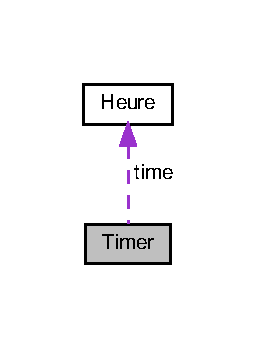
\includegraphics[width=124pt]{structTimer__coll__graph}
\end{center}
\end{figure}
\subsection*{Data Fields}
\begin{DoxyCompactItemize}
\item 
\mbox{\Hypertarget{structTimer_ad6e980d932698bb8fd82498e6c47696c}\label{structTimer_ad6e980d932698bb8fd82498e6c47696c}} 
int {\bfseries start\+Ticks}
\item 
\mbox{\Hypertarget{structTimer_a656a26aa06175d577077ac6181e772fd}\label{structTimer_a656a26aa06175d577077ac6181e772fd}} 
int {\bfseries paused\+Ticks}
\item 
\mbox{\Hypertarget{structTimer_a7fb9c61c8c6b3277fa1a33a054987704}\label{structTimer_a7fb9c61c8c6b3277fa1a33a054987704}} 
int {\bfseries paused}
\item 
\mbox{\Hypertarget{structTimer_ae61fe29f9f0ed5eb7eed278b3dee29f0}\label{structTimer_ae61fe29f9f0ed5eb7eed278b3dee29f0}} 
int {\bfseries started}
\item 
\mbox{\Hypertarget{structTimer_ac7f0cfc2a6dadae0951dd728c60eba69}\label{structTimer_ac7f0cfc2a6dadae0951dd728c60eba69}} 
\hyperlink{structheure}{heure} {\bfseries time}
\end{DoxyCompactItemize}


The documentation for this struct was generated from the following file\+:\begin{DoxyCompactItemize}
\item 
background.\+h\end{DoxyCompactItemize}

\hypertarget{structtimer}{}\section{timer Struct Reference}
\label{structtimer}\index{timer@{timer}}


to count the time  




{\ttfamily \#include $<$background.\+h$>$}



\subsection{Detailed Description}
to count the time 

The documentation for this struct was generated from the following file\+:\begin{DoxyCompactItemize}
\item 
background.\+h\end{DoxyCompactItemize}

\hypertarget{structType}{}\section{Type Struct Reference}
\label{structType}\index{Type@{Type}}


the collision type  




{\ttfamily \#include $<$entite\+\_\+secondaire.\+h$>$}



\subsection{Detailed Description}
the collision type 

The documentation for this struct was generated from the following file\+:\begin{DoxyCompactItemize}
\item 
entite\+\_\+secondaire.\+h\end{DoxyCompactItemize}

\hypertarget{structVie}{}\section{Vie Struct Reference}
\label{structVie}\index{Vie@{Vie}}


For life parameters.  




{\ttfamily \#include $<$hero.\+h$>$}

\subsection*{Data Fields}
\begin{DoxyCompactItemize}
\item 
\mbox{\Hypertarget{structVie_a2656effa8772d33fe9d4d52212db99dc}\label{structVie_a2656effa8772d33fe9d4d52212db99dc}} 
S\+D\+L\+\_\+\+Surface $\ast$ {\bfseries heart}
\item 
\mbox{\Hypertarget{structVie_a7076ab45d1bad6fef6159b35d8056109}\label{structVie_a7076ab45d1bad6fef6159b35d8056109}} 
S\+D\+L\+\_\+\+Rect {\bfseries position\+\_\+heart\+\_\+a}
\item 
\mbox{\Hypertarget{structVie_ac0fc02d542c34723253eeca8cf4b8125}\label{structVie_ac0fc02d542c34723253eeca8cf4b8125}} 
S\+D\+L\+\_\+\+Rect {\bfseries position\+\_\+heart\+\_\+b}
\item 
\mbox{\Hypertarget{structVie_a0398326a6888247e76c1669bf2cd9d11}\label{structVie_a0398326a6888247e76c1669bf2cd9d11}} 
S\+D\+L\+\_\+\+Rect {\bfseries position\+\_\+heart\+\_\+c}
\item 
\mbox{\Hypertarget{structVie_a133255bdd7e91d9c2d90eaf71239540d}\label{structVie_a133255bdd7e91d9c2d90eaf71239540d}} 
int {\bfseries nb\+\_\+vie}
\end{DoxyCompactItemize}


\subsection{Detailed Description}
For life parameters. 

The documentation for this struct was generated from the following file\+:\begin{DoxyCompactItemize}
\item 
hero.\+h\end{DoxyCompactItemize}

\chapter{File Documentation}
\hypertarget{background_8c}{}\section{background.\+c File Reference}
\label{background_8c}\index{background.\+c@{background.\+c}}
{\ttfamily \#include \char`\"{}background.\+h\char`\"{}}\newline
Include dependency graph for background.\+c\+:\nopagebreak
\begin{figure}[H]
\begin{center}
\leavevmode
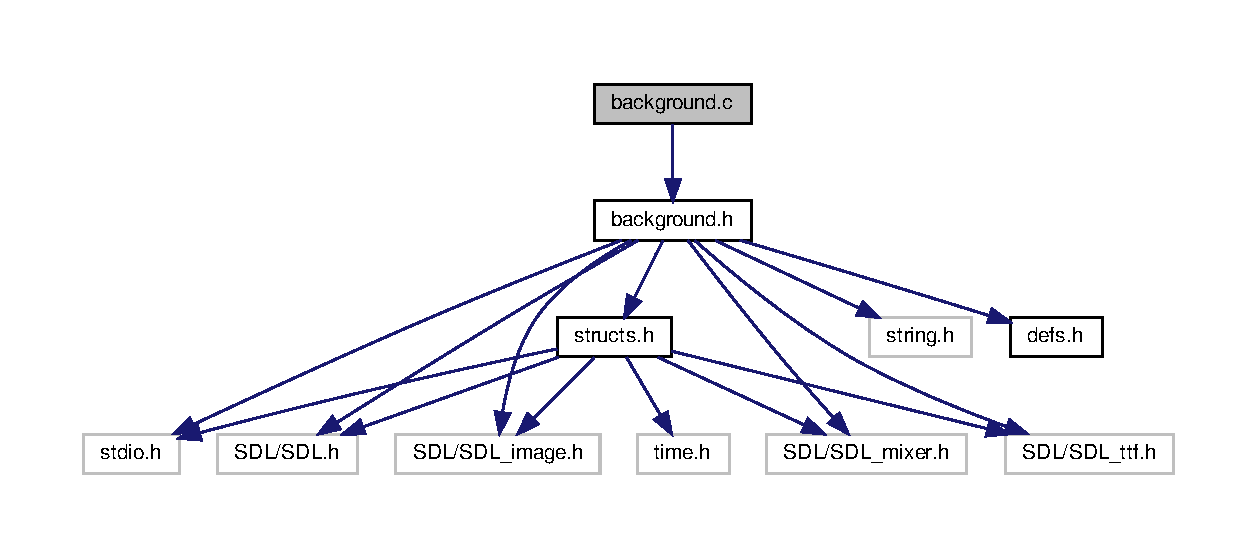
\includegraphics[width=350pt]{background_8c__incl}
\end{center}
\end{figure}
\subsection*{Functions}
\begin{DoxyCompactItemize}
\item 
\mbox{\Hypertarget{background_8c_afba44a2edceab261b24e39f7b88ac2a7}\label{background_8c_afba44a2edceab261b24e39f7b88ac2a7}} 
void {\bfseries initialiser\+\_\+background} (\hyperlink{structbackground}{background} $\ast$b, \hyperlink{structparameter}{parameter} p)
\item 
\mbox{\Hypertarget{background_8c_ad8a5f7044fd773576c1e552c6ad2deb5}\label{background_8c_ad8a5f7044fd773576c1e552c6ad2deb5}} 
void {\bfseries initialiser\+\_\+platforme} (\hyperlink{structplatforme}{platforme} $\ast$p, int x, int y, int interval, int sens)
\item 
\mbox{\Hypertarget{background_8c_a25def9009f384b9250988b9d4ec7f912}\label{background_8c_a25def9009f384b9250988b9d4ec7f912}} 
void {\bfseries initialiser\+\_\+plats} (\hyperlink{structplatforme}{platforme} plats\mbox{[}$\,$\mbox{]}, int n)
\item 
\mbox{\Hypertarget{background_8c_acbfe951965300d621d9aa29f5acef262}\label{background_8c_acbfe951965300d621d9aa29f5acef262}} 
void {\bfseries initialiser\+\_\+plats\+\_\+horiz} (\hyperlink{structplatforme}{platforme} plats\mbox{[}$\,$\mbox{]}, int n)
\item 
\mbox{\Hypertarget{background_8c_a4572c5affffdb5081fdb8d5671e0c99e}\label{background_8c_a4572c5affffdb5081fdb8d5671e0c99e}} 
void {\bfseries initialiser\+\_\+text} (\hyperlink{structtext}{text} $\ast$i, char message\mbox{[}40\mbox{]}, int x, int y, int size)
\item 
\mbox{\Hypertarget{background_8c_a101d9ea4b3eb68c5eb3e0d9ace4e3ff5}\label{background_8c_a101d9ea4b3eb68c5eb3e0d9ace4e3ff5}} 
void {\bfseries initialiser\+\_\+text\+\_\+2} (\hyperlink{structtext}{text} $\ast$i, int x, int y, int size)
\item 
\mbox{\Hypertarget{background_8c_ab444db3d8a148587e6f79636838d7bf3}\label{background_8c_ab444db3d8a148587e6f79636838d7bf3}} 
void {\bfseries initialiser\+\_\+instructions} (\hyperlink{structtext}{text} instructions\mbox{[}$\,$\mbox{]}, int n)
\item 
\mbox{\Hypertarget{background_8c_a563d6825cf533cfd17bfca200724ef18}\label{background_8c_a563d6825cf533cfd17bfca200724ef18}} 
void {\bfseries afficher\+\_\+background} (\hyperlink{structbackground}{background} $\ast$b, S\+D\+L\+\_\+\+Surface $\ast$screen)
\item 
\mbox{\Hypertarget{background_8c_a7820a8b06ca3cb672bbf4f0f82626efb}\label{background_8c_a7820a8b06ca3cb672bbf4f0f82626efb}} 
void {\bfseries afficher\+\_\+platformes} (\hyperlink{structplatforme}{platforme} plats\mbox{[}$\,$\mbox{]}, \hyperlink{structbackground}{background} b, S\+D\+L\+\_\+\+Surface $\ast$ecran, int n)
\item 
\mbox{\Hypertarget{background_8c_aa36b26f2e6c912c37bdcc22faf7ab81a}\label{background_8c_aa36b26f2e6c912c37bdcc22faf7ab81a}} 
void {\bfseries afficher\+\_\+text} (\hyperlink{structtext}{text} i, \hyperlink{structbackground}{background} b, S\+D\+L\+\_\+\+Surface $\ast$ecran)
\item 
\mbox{\Hypertarget{background_8c_a95ed33edf22a014868fd7ba6c0fcb331}\label{background_8c_a95ed33edf22a014868fd7ba6c0fcb331}} 
void {\bfseries afficher\+\_\+text\+\_\+2} (\hyperlink{structtext}{text} i, S\+D\+L\+\_\+\+Surface $\ast$ecran, char message\mbox{[}20\mbox{]})
\item 
\mbox{\Hypertarget{background_8c_a51011f31a342be5d21889da00baa2b21}\label{background_8c_a51011f31a342be5d21889da00baa2b21}} 
void {\bfseries afficher\+\_\+instructions} (\hyperlink{structtext}{text} instructions\mbox{[}$\,$\mbox{]}, int n, \hyperlink{structbackground}{background} b, S\+D\+L\+\_\+\+Surface $\ast$ecran)
\item 
\mbox{\Hypertarget{background_8c_aa67f7366249fded07e59818c618a8a21}\label{background_8c_aa67f7366249fded07e59818c618a8a21}} 
void {\bfseries animer\+\_\+platformes} (\hyperlink{structplatforme}{platforme} plats\mbox{[}$\,$\mbox{]}, int n)
\item 
\mbox{\Hypertarget{background_8c_a1c83a94deca8f75cfce4e94c6f4afe84}\label{background_8c_a1c83a94deca8f75cfce4e94c6f4afe84}} 
void {\bfseries animer\+\_\+platformes\+\_\+horiz} (\hyperlink{structplatforme}{platforme} plats\mbox{[}$\,$\mbox{]}, int n)
\item 
\mbox{\Hypertarget{background_8c_aaaf5d97d125ff860ec566fe1a36c4155}\label{background_8c_aaaf5d97d125ff860ec566fe1a36c4155}} 
void {\bfseries init\+\_\+timer} (\hyperlink{structtimer}{timer} $\ast$t)
\item 
\mbox{\Hypertarget{background_8c_ae951bc4acad582d20531e64af771854a}\label{background_8c_ae951bc4acad582d20531e64af771854a}} 
void {\bfseries start\+\_\+timer} (\hyperlink{structtimer}{timer} $\ast$t)
\item 
\mbox{\Hypertarget{background_8c_a13ed51da8181b8dac5dbb44f3877c71c}\label{background_8c_a13ed51da8181b8dac5dbb44f3877c71c}} 
void {\bfseries stop\+\_\+timer} (\hyperlink{structtimer}{timer} $\ast$t)
\item 
\mbox{\Hypertarget{background_8c_afa1bde0a1ef2ad4e9884e1b2d09cebe0}\label{background_8c_afa1bde0a1ef2ad4e9884e1b2d09cebe0}} 
void {\bfseries get\+\_\+time} (\hyperlink{structtimer}{timer} $\ast$t)
\item 
\mbox{\Hypertarget{background_8c_a08d11897041bea6ecc93a79a2ac2e0b9}\label{background_8c_a08d11897041bea6ecc93a79a2ac2e0b9}} 
void {\bfseries pause\+\_\+timer} (\hyperlink{structtimer}{timer} $\ast$t)
\item 
\mbox{\Hypertarget{background_8c_a84dcfedfe1b26b3dcbf304566a73cb39}\label{background_8c_a84dcfedfe1b26b3dcbf304566a73cb39}} 
void {\bfseries resume\+\_\+timer} (\hyperlink{structtimer}{timer} $\ast$t)
\item 
\mbox{\Hypertarget{background_8c_a80322bf1b6a09e48eeba2f15ffbcca1a}\label{background_8c_a80322bf1b6a09e48eeba2f15ffbcca1a}} 
void {\bfseries show\+\_\+time} (\hyperlink{structtimer}{timer} $\ast$t, S\+D\+L\+\_\+\+Surface $\ast$screen)
\item 
\mbox{\Hypertarget{background_8c_acd5c391fb21c6fc46a4f71e48749a8d8}\label{background_8c_acd5c391fb21c6fc46a4f71e48749a8d8}} 
void {\bfseries afficher\+\_\+temps} (\hyperlink{structtext}{text} $\ast$t, \hyperlink{structtimer}{timer} $\ast$\hyperlink{structtimer}{timer}, S\+D\+L\+\_\+\+Surface $\ast$ecran)
\item 
\mbox{\Hypertarget{background_8c_a1965ff2d66416eb113acbbfbe859f77a}\label{background_8c_a1965ff2d66416eb113acbbfbe859f77a}} 
void {\bfseries free\+\_\+param} (\hyperlink{structparameter}{parameter} $\ast$p)
\item 
\mbox{\Hypertarget{background_8c_a1c93ad11c466554f9d89605d7b8ede7b}\label{background_8c_a1c93ad11c466554f9d89605d7b8ede7b}} 
void {\bfseries free\+\_\+background} (\hyperlink{structbackground}{background} $\ast$b)
\item 
\mbox{\Hypertarget{background_8c_af51c2f8a2ecb21de3ae567f11518b6c9}\label{background_8c_af51c2f8a2ecb21de3ae567f11518b6c9}} 
void {\bfseries free\+\_\+platformes} (\hyperlink{structplatforme}{platforme} plats\mbox{[}$\,$\mbox{]}, int n)
\item 
\mbox{\Hypertarget{background_8c_ac991590a05c5b13cd632606ff2ee6d1f}\label{background_8c_ac991590a05c5b13cd632606ff2ee6d1f}} 
void {\bfseries free\+\_\+instructions} (\hyperlink{structtext}{text} instructions\mbox{[}$\,$\mbox{]}, int n)
\end{DoxyCompactItemize}

\hypertarget{collision_8c}{}\section{collision.\+c File Reference}
\label{collision_8c}\index{collision.\+c@{collision.\+c}}
{\ttfamily \#include \char`\"{}collision.\+h\char`\"{}}\newline
Include dependency graph for collision.\+c\+:\nopagebreak
\begin{figure}[H]
\begin{center}
\leavevmode
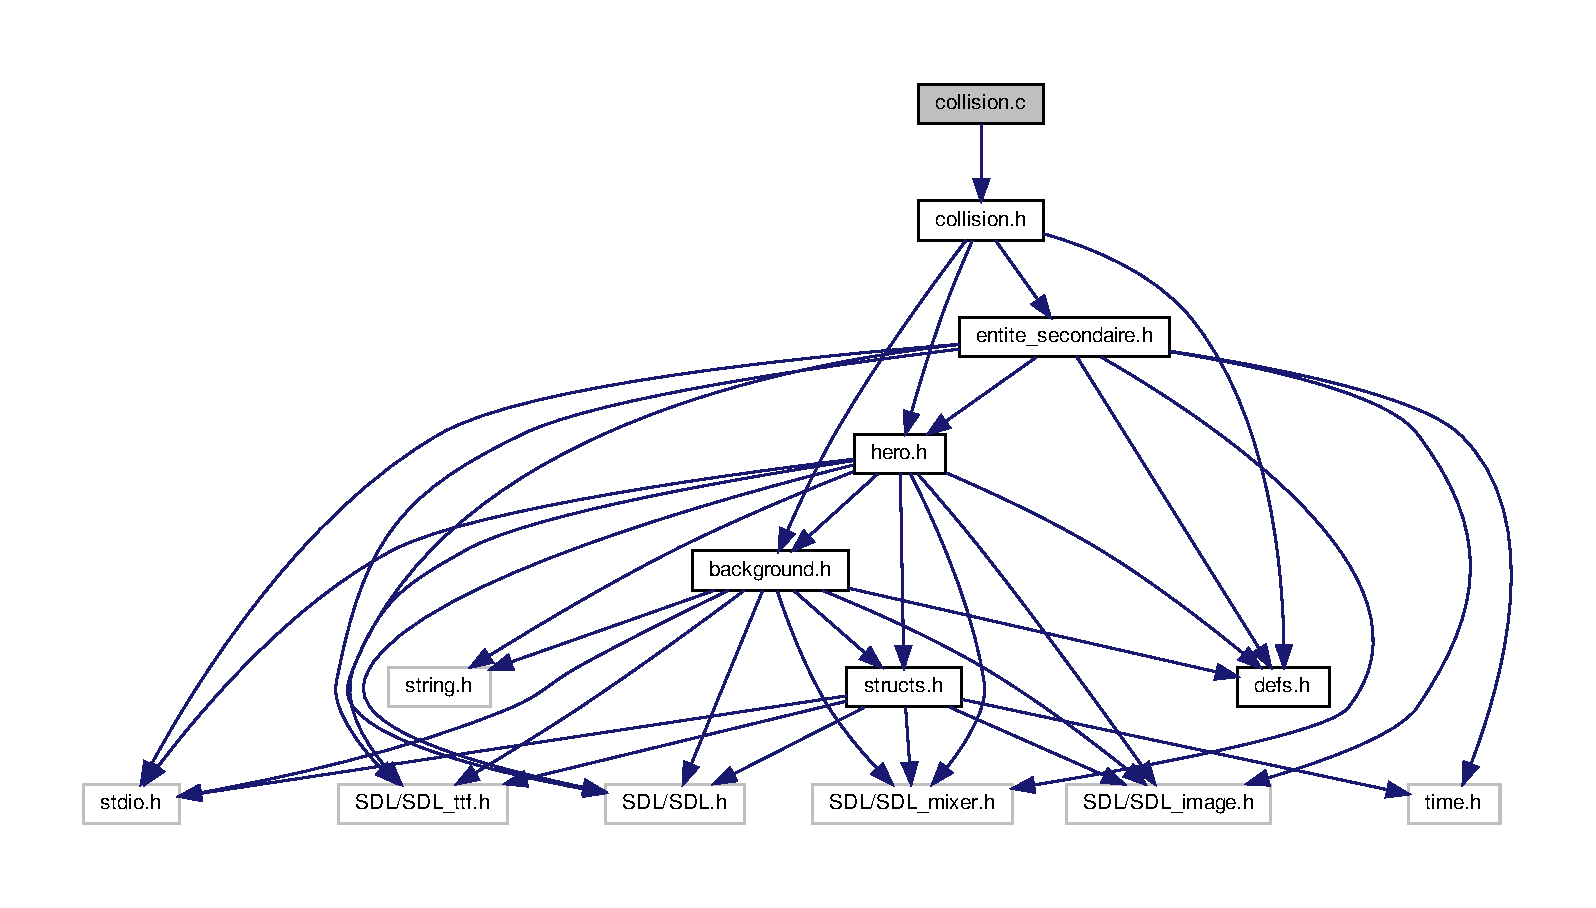
\includegraphics[width=350pt]{collision_8c__incl}
\end{center}
\end{figure}
\subsection*{Functions}
\begin{DoxyCompactItemize}
\item 
\mbox{\Hypertarget{collision_8c_a9ec79b71532402381966fc93325d3e52}\label{collision_8c_a9ec79b71532402381966fc93325d3e52}} 
S\+D\+L\+\_\+\+Color {\bfseries Get\+Pixel} (S\+D\+L\+\_\+\+Surface $\ast$p\+Surface, int x, int y)
\item 
\mbox{\Hypertarget{collision_8c_a4a38df492988109d6b404de7a542c3ce}\label{collision_8c_a4a38df492988109d6b404de7a542c3ce}} 
void {\bfseries Collision\+Parfaite} (\hyperlink{structHero}{hero} $\ast$h, \hyperlink{structbackground}{background} b)
\item 
\mbox{\Hypertarget{collision_8c_ae3894b92f2cdc9c72d7e04b697e68144}\label{collision_8c_ae3894b92f2cdc9c72d7e04b697e68144}} 
int {\bfseries collision\+\_\+platforme} (\hyperlink{structHero}{hero} $\ast$h, \hyperlink{structplatforme}{platforme} plats\mbox{[}$\,$\mbox{]}, int n)
\item 
\mbox{\Hypertarget{collision_8c_acc249ee2930f338cb741b24a57f129eb}\label{collision_8c_acc249ee2930f338cb741b24a57f129eb}} 
int {\bfseries collision\+\_\+platforme2} (\hyperlink{structHero}{hero} $\ast$h, \hyperlink{structplatforme}{platforme} plats\mbox{[}$\,$\mbox{]}, int n)
\item 
\mbox{\Hypertarget{collision_8c_ab3fcb69f51fd9ff709abf655d99f8505}\label{collision_8c_ab3fcb69f51fd9ff709abf655d99f8505}} 
int {\bfseries collision} (\hyperlink{structEntite}{entite} $\ast$e, \hyperlink{structHero}{hero} $\ast$h)
\item 
\mbox{\Hypertarget{collision_8c_a29f022801abe7ec63f220bb80760f809}\label{collision_8c_a29f022801abe7ec63f220bb80760f809}} 
int {\bfseries collision\+\_\+boss} (\hyperlink{structBoss}{boss} $\ast$e, \hyperlink{structHero}{hero} $\ast$h)
\end{DoxyCompactItemize}

\hypertarget{enigme__match_8c}{}\section{enigme\+\_\+match.\+c File Reference}
\label{enigme__match_8c}\index{enigme\+\_\+match.\+c@{enigme\+\_\+match.\+c}}
{\ttfamily \#include \char`\"{}matchsticks.\+h\char`\"{}}\newline
{\ttfamily \#include \char`\"{}background.\+h\char`\"{}}\newline
{\ttfamily \#include \char`\"{}hero.\+h\char`\"{}}\newline
Include dependency graph for enigme\+\_\+match.\+c\+:\nopagebreak
\begin{figure}[H]
\begin{center}
\leavevmode
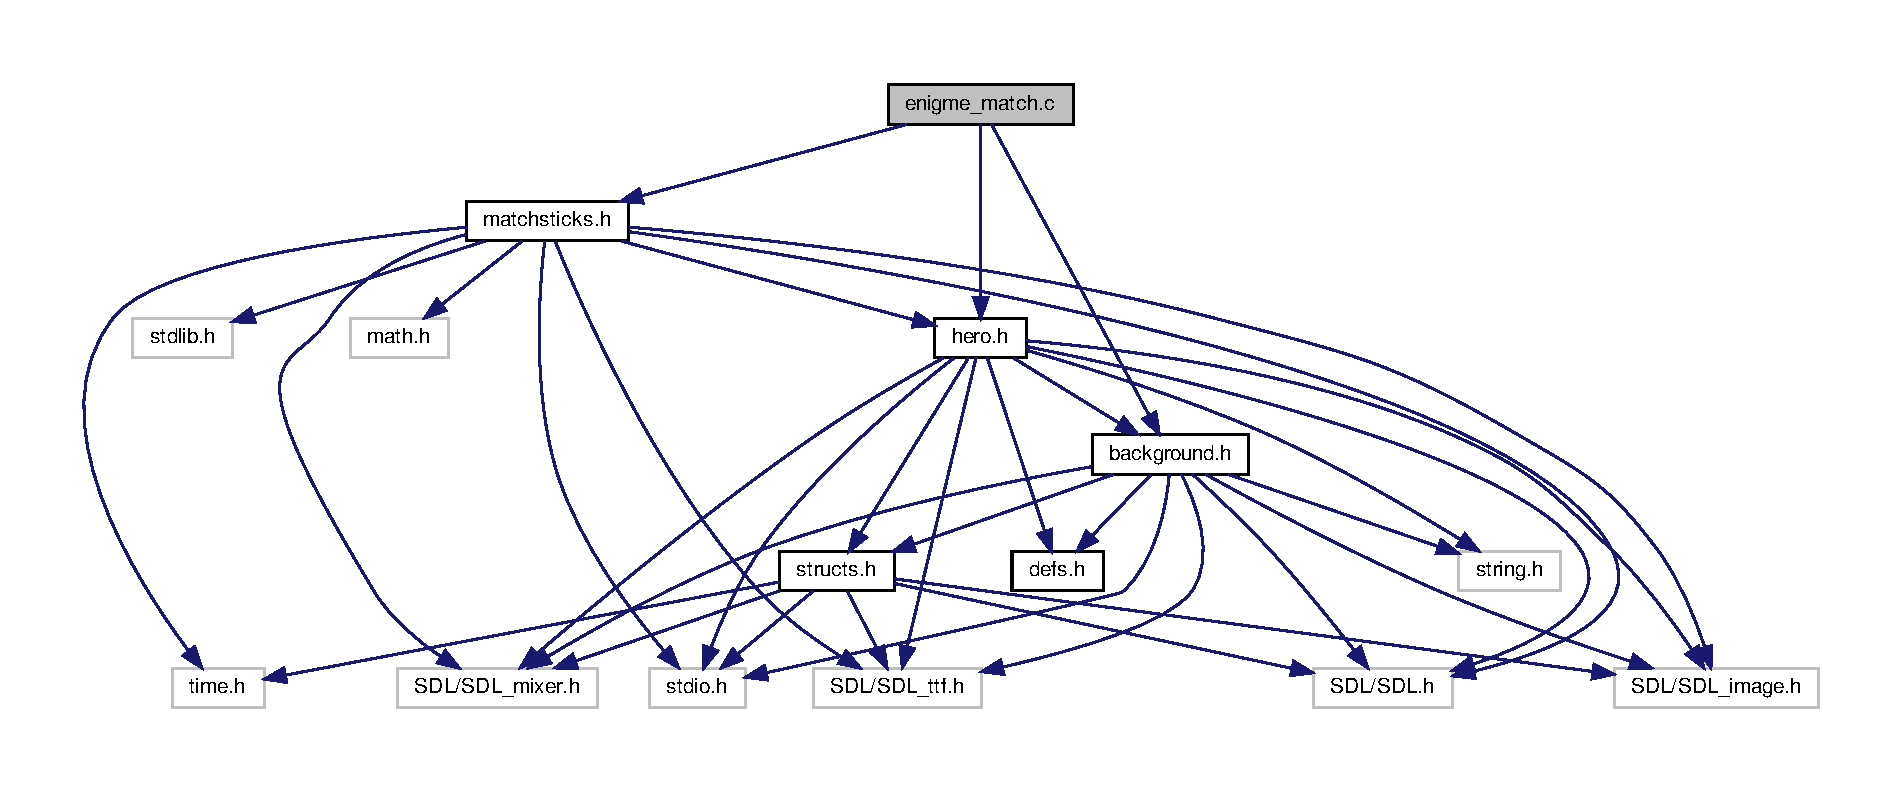
\includegraphics[width=350pt]{enigme__match_8c__incl}
\end{center}
\end{figure}
\subsection*{Functions}
\begin{DoxyCompactItemize}
\item 
\mbox{\Hypertarget{enigme__match_8c_ad2aedfd0ef0b4ffd9b1fa83eec18ec8c}\label{enigme__match_8c_ad2aedfd0ef0b4ffd9b1fa83eec18ec8c}} 
void {\bfseries initialiser\+\_\+text\+\_\+enigme} (\hyperlink{structText__enigme}{text\+\_\+enigme} $\ast$i, char message\mbox{[}40\mbox{]}, int x, int y, int size)
\item 
\mbox{\Hypertarget{enigme__match_8c_ac7dfc55563600d252c9b3adfeee59918}\label{enigme__match_8c_ac7dfc55563600d252c9b3adfeee59918}} 
void {\bfseries afficher\+\_\+text\+\_\+enigme} (\hyperlink{structText__enigme}{text\+\_\+enigme} i, S\+D\+L\+\_\+\+Surface $\ast$ecran, char message\mbox{[}20\mbox{]})
\item 
\mbox{\Hypertarget{enigme__match_8c_ac81145beb0b07141617c561c7eba5102}\label{enigme__match_8c_ac81145beb0b07141617c561c7eba5102}} 
int {\bfseries rand\+\_\+matchs} (int Match\+Count)
\item 
\mbox{\Hypertarget{enigme__match_8c_a8df6166b1af575a8af08c1ad6fe4e736}\label{enigme__match_8c_a8df6166b1af575a8af08c1ad6fe4e736}} 
void {\bfseries Init} (\hyperlink{structText__enigme}{text\+\_\+enigme} $\ast$match\+Text, \hyperlink{structText__enigme}{text\+\_\+enigme} $\ast$Pturn\+Text, \hyperlink{structText__enigme}{text\+\_\+enigme} $\ast$A\+Iturn\+Text, \hyperlink{structMatchstick}{Matchstick} $\ast$match)
\item 
\mbox{\Hypertarget{enigme__match_8c_a9f3c14e67cec924709f10cfadba03e5e}\label{enigme__match_8c_a9f3c14e67cec924709f10cfadba03e5e}} 
void {\bfseries affichage\+\_\+matchs} (S\+D\+L\+\_\+\+Surface $\ast$screen, \hyperlink{structMatchstick}{Matchstick} $\ast$match)
\item 
\mbox{\Hypertarget{enigme__match_8c_addef751480273e3fc408417118518f4f}\label{enigme__match_8c_addef751480273e3fc408417118518f4f}} 
void {\bfseries update\+Text} (S\+D\+L\+\_\+\+Surface $\ast$screen, int turn, \hyperlink{structText__enigme}{text\+\_\+enigme} $\ast$Pturn\+Text, \hyperlink{structText__enigme}{text\+\_\+enigme} $\ast$A\+Iturn\+Text)
\item 
\mbox{\Hypertarget{enigme__match_8c_ac00162d87efd3ddb5079ff605571bbef}\label{enigme__match_8c_ac00162d87efd3ddb5079ff605571bbef}} 
void {\bfseries afficher\+Text} (S\+D\+L\+\_\+\+Surface $\ast$screen, \hyperlink{structText__enigme}{text\+\_\+enigme} matchtext, \hyperlink{structText__enigme}{text\+\_\+enigme} Pturn\+Text, \hyperlink{structText__enigme}{text\+\_\+enigme} A\+Iturn\+Text, int turn)
\item 
\mbox{\Hypertarget{enigme__match_8c_a976fe143b8d95318705e426e1b3b0ba3}\label{enigme__match_8c_a976fe143b8d95318705e426e1b3b0ba3}} 
void {\bfseries game\+\_\+end} (\hyperlink{structMatchstick}{Matchstick} match, int Turn, \hyperlink{structText__enigme}{text\+\_\+enigme} $\ast$Pturn\+Text, \hyperlink{structText__enigme}{text\+\_\+enigme} $\ast$A\+Iturn\+Text, int $\ast$A\+Icontinuer, int $\ast$win)
\item 
\mbox{\Hypertarget{enigme__match_8c_ae982e631730163f723d9ad3f4085bb28}\label{enigme__match_8c_ae982e631730163f723d9ad3f4085bb28}} 
int {\bfseries A\+I\+\_\+enigme} (S\+D\+L\+\_\+\+Surface $\ast$screen, \hyperlink{structHero}{hero} $\ast$h)
\end{DoxyCompactItemize}

\hypertarget{enigme__math_8c}{}\section{enigme\+\_\+math.\+c File Reference}
\label{enigme__math_8c}\index{enigme\+\_\+math.\+c@{enigme\+\_\+math.\+c}}
{\ttfamily \#include \char`\"{}enigme.\+h\char`\"{}}\newline
{\ttfamily \#include \char`\"{}hero.\+h\char`\"{}}\newline
Include dependency graph for enigme\+\_\+math.\+c\+:\nopagebreak
\begin{figure}[H]
\begin{center}
\leavevmode
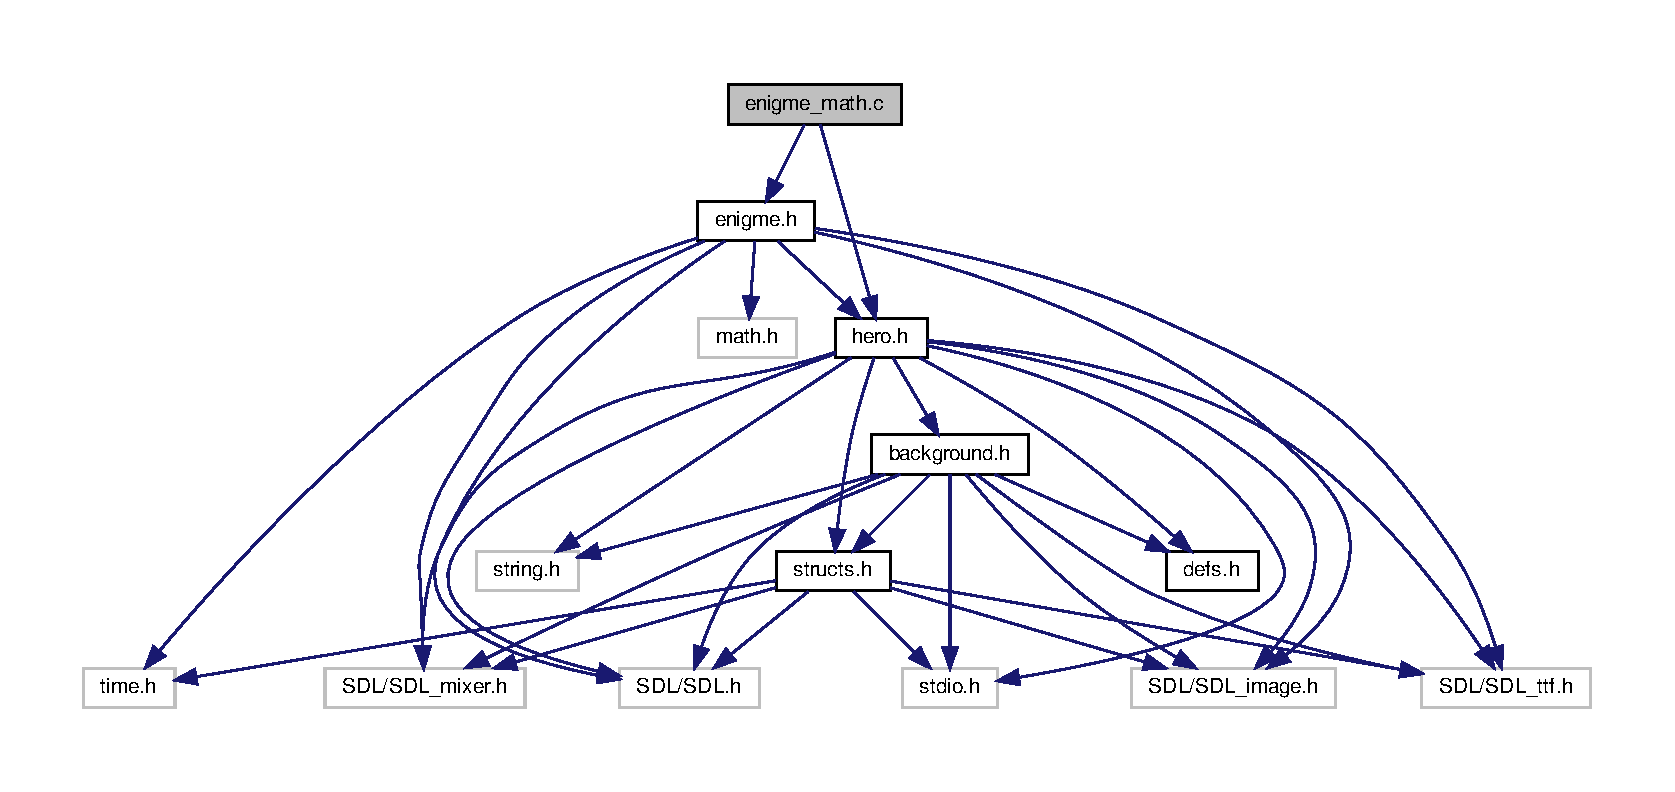
\includegraphics[width=350pt]{enigme__math_8c__incl}
\end{center}
\end{figure}
\subsection*{Functions}
\begin{DoxyCompactItemize}
\item 
\mbox{\Hypertarget{enigme__math_8c_a32b1be1bc3bcad4b54df04fccb52184c}\label{enigme__math_8c_a32b1be1bc3bcad4b54df04fccb52184c}} 
void {\bfseries enigme\+\_\+math} (S\+D\+L\+\_\+\+Surface $\ast$screen, \hyperlink{structenigme}{enigme} $\ast$E, \hyperlink{structHero}{hero} $\ast$h)
\end{DoxyCompactItemize}

\hypertarget{enigme__pendu_8c}{}\section{enigme\+\_\+pendu.\+c File Reference}
\label{enigme__pendu_8c}\index{enigme\+\_\+pendu.\+c@{enigme\+\_\+pendu.\+c}}
{\ttfamily \#include \char`\"{}pendu.\+h\char`\"{}}\newline
Include dependency graph for enigme\+\_\+pendu.\+c\+:\nopagebreak
\begin{figure}[H]
\begin{center}
\leavevmode
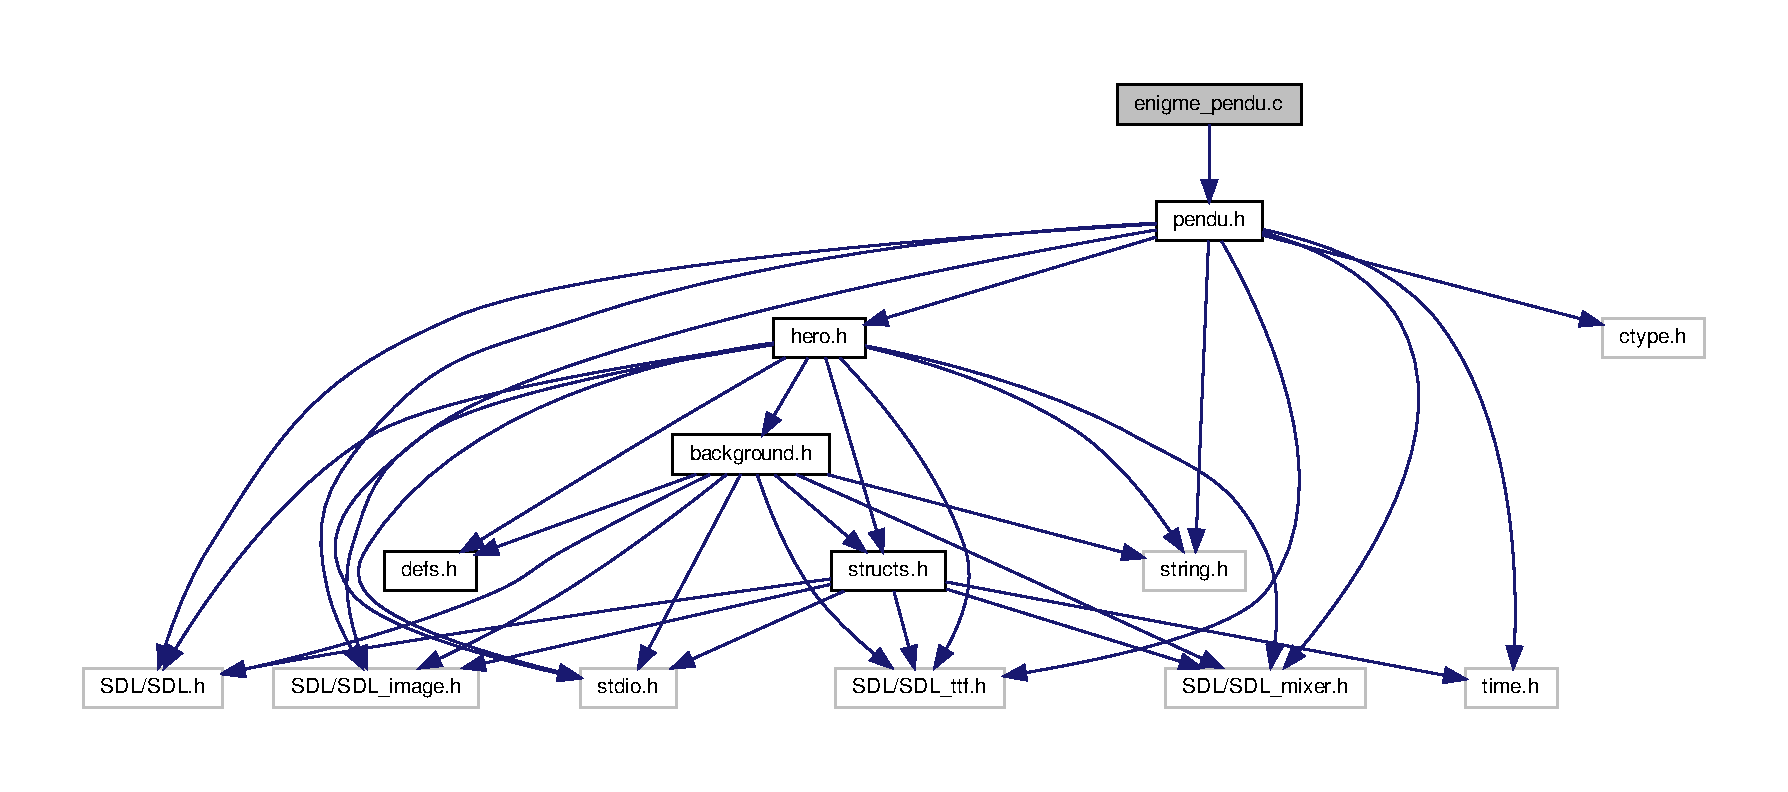
\includegraphics[width=350pt]{enigme__pendu_8c__incl}
\end{center}
\end{figure}
\subsection*{Functions}
\begin{DoxyCompactItemize}
\item 
\mbox{\Hypertarget{enigme__pendu_8c_af0136c24c92dbfbf7514567d85fe6a4b}\label{enigme__pendu_8c_af0136c24c92dbfbf7514567d85fe6a4b}} 
int {\bfseries enigme\+\_\+pendu} (S\+D\+L\+\_\+\+Surface $\ast$screen, \hyperlink{structHero}{hero} $\ast$h)
\end{DoxyCompactItemize}

\hypertarget{entite__secondaire_8c}{}\section{entite\+\_\+secondaire.\+c File Reference}
\label{entite__secondaire_8c}\index{entite\+\_\+secondaire.\+c@{entite\+\_\+secondaire.\+c}}
{\ttfamily \#include \char`\"{}entite\+\_\+secondaire.\+h\char`\"{}}\newline
{\ttfamily \#include \char`\"{}collision.\+h\char`\"{}}\newline
Include dependency graph for entite\+\_\+secondaire.\+c\+:\nopagebreak
\begin{figure}[H]
\begin{center}
\leavevmode
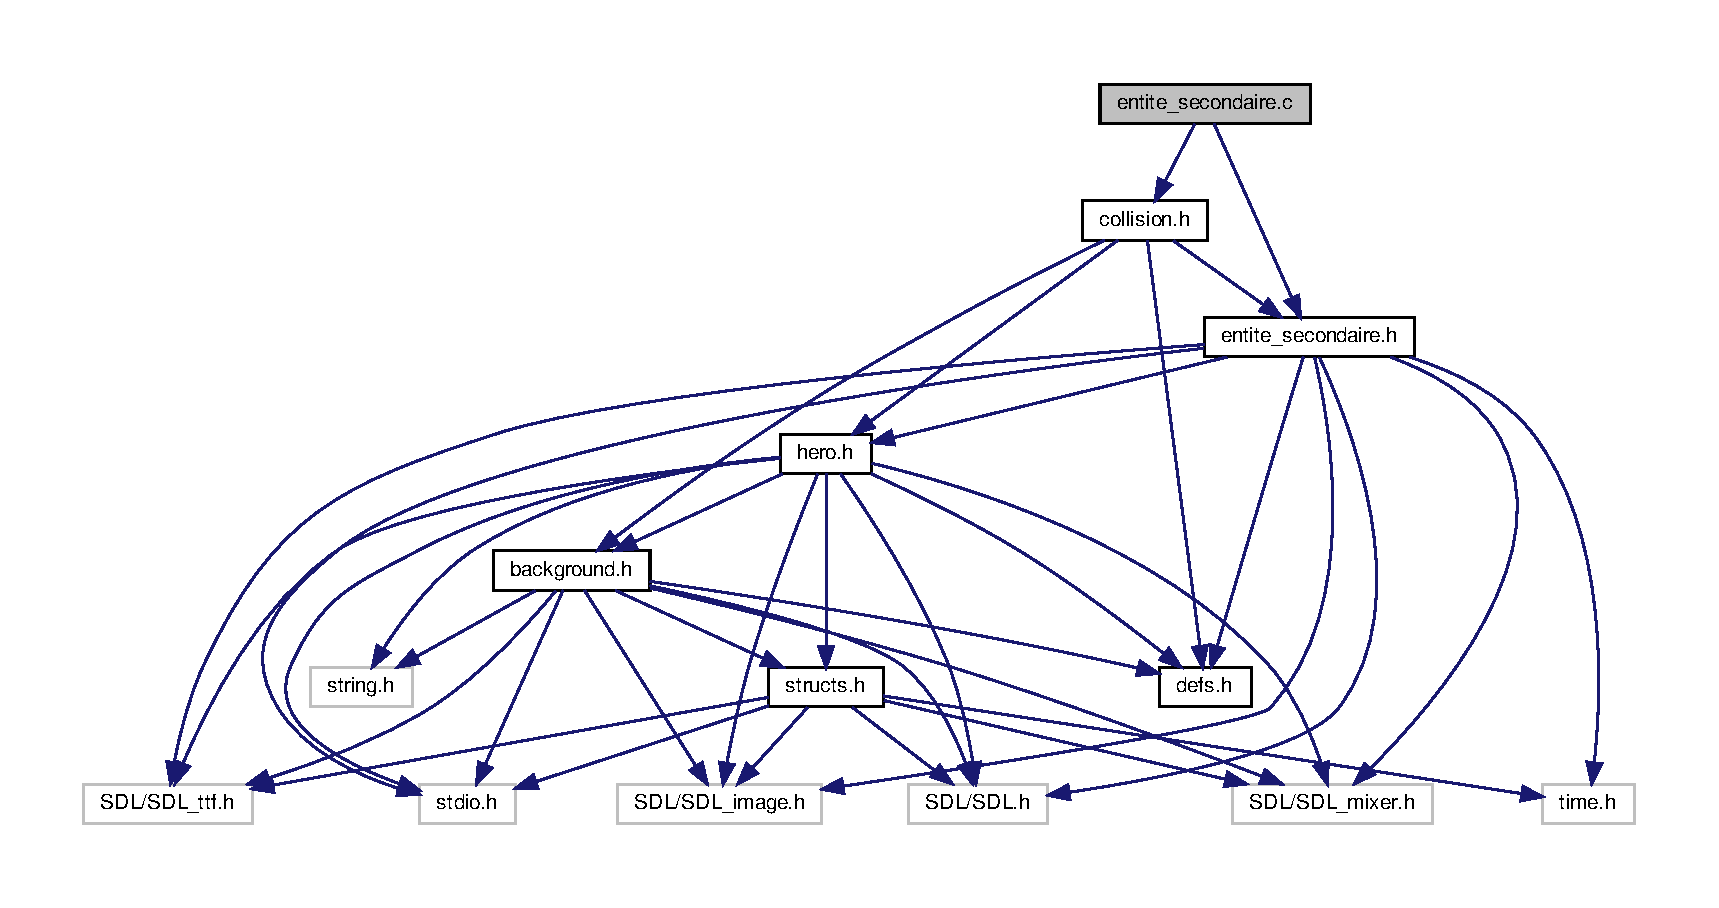
\includegraphics[width=350pt]{entite__secondaire_8c__incl}
\end{center}
\end{figure}
\subsection*{Functions}
\begin{DoxyCompactItemize}
\item 
\mbox{\Hypertarget{entite__secondaire_8c_ae1d3bb91a5272b11f930d9343db34bef}\label{entite__secondaire_8c_ae1d3bb91a5272b11f930d9343db34bef}} 
void {\bfseries initialiser\+\_\+entite} (\hyperlink{structEntite}{entite} $\ast$E, int x, int y)
\item 
\mbox{\Hypertarget{entite__secondaire_8c_a46315753d098981997cbeae55cfb5805}\label{entite__secondaire_8c_a46315753d098981997cbeae55cfb5805}} 
void {\bfseries initialiser\+\_\+ennemies} (\hyperlink{structEntite}{entite} tab\mbox{[}$\,$\mbox{]}, int n)
\item 
\mbox{\Hypertarget{entite__secondaire_8c_abb87afb394e5afe608ce66038f32702f}\label{entite__secondaire_8c_abb87afb394e5afe608ce66038f32702f}} 
void {\bfseries animer\+\_\+ennemies} (\hyperlink{structEntite}{entite} tab\mbox{[}$\,$\mbox{]}, int n)
\item 
\mbox{\Hypertarget{entite__secondaire_8c_aa8756a90975917347bfb0dfdec04b2b2}\label{entite__secondaire_8c_aa8756a90975917347bfb0dfdec04b2b2}} 
void {\bfseries deplacer\+\_\+alea\+\_\+ennemies} (\hyperlink{structEntite}{entite} tab\mbox{[}$\,$\mbox{]}, int n)
\item 
\mbox{\Hypertarget{entite__secondaire_8c_a2481dcbb4aebcae6a332cdf53929f2ee}\label{entite__secondaire_8c_a2481dcbb4aebcae6a332cdf53929f2ee}} 
void {\bfseries attack\+\_\+ennemies} (\hyperlink{structEntite}{entite} tab\mbox{[}$\,$\mbox{]}, int n, \hyperlink{structHero}{hero} $\ast$h)
\item 
\mbox{\Hypertarget{entite__secondaire_8c_aaa2e418724a73ebd74bb98dcd119f3ab}\label{entite__secondaire_8c_aaa2e418724a73ebd74bb98dcd119f3ab}} 
void {\bfseries free\+\_\+ennemies} (\hyperlink{structEntite}{entite} tab\mbox{[}$\,$\mbox{]}, int n)
\item 
\mbox{\Hypertarget{entite__secondaire_8c_aebca3eddd3b769df4cdfae2ec041aa6f}\label{entite__secondaire_8c_aebca3eddd3b769df4cdfae2ec041aa6f}} 
void {\bfseries afficher\+\_\+ennemies} (\hyperlink{structEntite}{entite} tab\mbox{[}$\,$\mbox{]}, int n, S\+D\+L\+\_\+\+Surface $\ast$screen, \hyperlink{structbackground}{background} b)
\item 
\mbox{\Hypertarget{entite__secondaire_8c_ae4f8bdf6cb871720e797b5fe9f7343b0}\label{entite__secondaire_8c_ae4f8bdf6cb871720e797b5fe9f7343b0}} 
void {\bfseries animer\+\_\+entite} (\hyperlink{structEntite}{entite} $\ast$E)
\item 
\mbox{\Hypertarget{entite__secondaire_8c_a0e7c635c7d9385ce92548d933eb6c983}\label{entite__secondaire_8c_a0e7c635c7d9385ce92548d933eb6c983}} 
void {\bfseries deplacer\+\_\+alea} (\hyperlink{structEntite}{entite} $\ast$E)
\item 
\mbox{\Hypertarget{entite__secondaire_8c_a8da89fe2a429400b898b6d1e645ffdef}\label{entite__secondaire_8c_a8da89fe2a429400b898b6d1e645ffdef}} 
void {\bfseries attack\+\_\+entite} (\hyperlink{structEntite}{entite} $\ast$E, \hyperlink{structHero}{hero} $\ast$h)
\item 
\mbox{\Hypertarget{entite__secondaire_8c_accd5f49d5019fc2fad5bdcf3b14c9b5e}\label{entite__secondaire_8c_accd5f49d5019fc2fad5bdcf3b14c9b5e}} 
void {\bfseries afficher\+\_\+entite} (\hyperlink{structEntite}{entite} $\ast$E, S\+D\+L\+\_\+\+Surface $\ast$screen, \hyperlink{structbackground}{background} b)
\item 
\mbox{\Hypertarget{entite__secondaire_8c_af23698c55f2adb009c6accb07eebec29}\label{entite__secondaire_8c_af23698c55f2adb009c6accb07eebec29}} 
void {\bfseries free\+\_\+entite} (\hyperlink{structEntite}{entite} $\ast$E)
\item 
\mbox{\Hypertarget{entite__secondaire_8c_a4e1eae58517810a71546a8ea9e731493}\label{entite__secondaire_8c_a4e1eae58517810a71546a8ea9e731493}} 
void {\bfseries initialiser\+\_\+coins} (\hyperlink{structpower__up}{power\+\_\+up} coins\mbox{[}$\,$\mbox{]}, int n)
\item 
\mbox{\Hypertarget{entite__secondaire_8c_aca19fe0421270832081ee8e4b206fd2f}\label{entite__secondaire_8c_aca19fe0421270832081ee8e4b206fd2f}} 
void {\bfseries coins\+\_\+interaction} (\hyperlink{structpower__up}{power\+\_\+up} coins\mbox{[}$\,$\mbox{]}, int n, \hyperlink{structHero}{hero} $\ast$h)
\item 
\mbox{\Hypertarget{entite__secondaire_8c_a1bd1a2ad7adc2bc0b79ee6283771201e}\label{entite__secondaire_8c_a1bd1a2ad7adc2bc0b79ee6283771201e}} 
void {\bfseries animer\+\_\+coins} (\hyperlink{structpower__up}{power\+\_\+up} coins\mbox{[}$\,$\mbox{]}, int n)
\item 
\mbox{\Hypertarget{entite__secondaire_8c_ae821188174d025e2d24bcadcf05555c9}\label{entite__secondaire_8c_ae821188174d025e2d24bcadcf05555c9}} 
void {\bfseries afficher\+\_\+coins} (\hyperlink{structpower__up}{power\+\_\+up} coins\mbox{[}$\,$\mbox{]}, int n, \hyperlink{structbackground}{background} b, S\+D\+L\+\_\+\+Surface $\ast$ecran)
\item 
\mbox{\Hypertarget{entite__secondaire_8c_ab1a7b33d4e1c9adb936d5d5457298dad}\label{entite__secondaire_8c_ab1a7b33d4e1c9adb936d5d5457298dad}} 
void {\bfseries init\+\_\+heart} (\hyperlink{structheart}{heart} $\ast$h, int x, int y)
\item 
\mbox{\Hypertarget{entite__secondaire_8c_aa456107db8baddd7ff0637a32042befc}\label{entite__secondaire_8c_aa456107db8baddd7ff0637a32042befc}} 
void {\bfseries initialiser\+\_\+hearts} (\hyperlink{structheart}{heart} hearts\mbox{[}$\,$\mbox{]}, int n)
\item 
\mbox{\Hypertarget{entite__secondaire_8c_a0fc0b09bb9b89a9580182691d727f20d}\label{entite__secondaire_8c_a0fc0b09bb9b89a9580182691d727f20d}} 
void {\bfseries animer\+\_\+hearts} (\hyperlink{structheart}{heart} hearts\mbox{[}$\,$\mbox{]}, int n)
\item 
\mbox{\Hypertarget{entite__secondaire_8c_ab1127e4debb7af3c5b98d61fc68010a4}\label{entite__secondaire_8c_ab1127e4debb7af3c5b98d61fc68010a4}} 
void {\bfseries hearts\+\_\+interaction} (\hyperlink{structheart}{heart} hearts\mbox{[}$\,$\mbox{]}, int n, \hyperlink{structHero}{hero} $\ast$h)
\item 
\mbox{\Hypertarget{entite__secondaire_8c_afeae549eab6326c93de767b0ef36c60a}\label{entite__secondaire_8c_afeae549eab6326c93de767b0ef36c60a}} 
void {\bfseries afficher\+\_\+hearts} (\hyperlink{structheart}{heart} hearts\mbox{[}$\,$\mbox{]}, int n, \hyperlink{structbackground}{background} b, S\+D\+L\+\_\+\+Surface $\ast$ecran)
\item 
\mbox{\Hypertarget{entite__secondaire_8c_a9b603c185eb8b595a3fa7920bb123e70}\label{entite__secondaire_8c_a9b603c185eb8b595a3fa7920bb123e70}} 
void {\bfseries free\+\_\+pu} (\hyperlink{structpower__up}{power\+\_\+up} p\mbox{[}$\,$\mbox{]}, int n)
\item 
\mbox{\Hypertarget{entite__secondaire_8c_a65962b886e2d1ac518294399cdfe36dc}\label{entite__secondaire_8c_a65962b886e2d1ac518294399cdfe36dc}} 
void {\bfseries free\+\_\+hearts} (\hyperlink{structheart}{heart} hearts\mbox{[}$\,$\mbox{]}, int n)
\item 
\mbox{\Hypertarget{entite__secondaire_8c_ab0196fce24ad36f0211231a1fa1561e7}\label{entite__secondaire_8c_ab0196fce24ad36f0211231a1fa1561e7}} 
void {\bfseries init\+\_\+mats} (\hyperlink{structMat}{mat} $\ast$e, \hyperlink{structMat}{mat} $\ast$c1, \hyperlink{structMat}{mat} $\ast$c2)
\item 
\mbox{\Hypertarget{entite__secondaire_8c_ac9a30398583fc2c35a685d025d3941f1}\label{entite__secondaire_8c_ac9a30398583fc2c35a685d025d3941f1}} 
void {\bfseries animer\+\_\+mat} (\hyperlink{structMat}{mat} $\ast$e, \hyperlink{structMat}{mat} $\ast$c1, \hyperlink{structMat}{mat} $\ast$c2)
\item 
\mbox{\Hypertarget{entite__secondaire_8c_a75ea7d18dad88bd47d01da05dc3c1012}\label{entite__secondaire_8c_a75ea7d18dad88bd47d01da05dc3c1012}} 
void {\bfseries collision\+\_\+mat} (\hyperlink{structHero}{hero} $\ast$h, \hyperlink{structMat}{mat} e, \hyperlink{structMat}{mat} c1, \hyperlink{structMat}{mat} c2)
\item 
\mbox{\Hypertarget{entite__secondaire_8c_a1cb442c301628b9d3639d4fefbfa7607}\label{entite__secondaire_8c_a1cb442c301628b9d3639d4fefbfa7607}} 
void {\bfseries afficher\+\_\+mat} (\hyperlink{structMat}{mat} e, \hyperlink{structMat}{mat} c1, \hyperlink{structMat}{mat} c2, \hyperlink{structbackground}{background} b, S\+D\+L\+\_\+\+Surface $\ast$screen)
\item 
\mbox{\Hypertarget{entite__secondaire_8c_aac869d62607a482fe635f3e7c9b8cca4}\label{entite__secondaire_8c_aac869d62607a482fe635f3e7c9b8cca4}} 
void {\bfseries init\+\_\+boss} (\hyperlink{structBoss}{boss} $\ast$E, int x, int y)
\item 
\mbox{\Hypertarget{entite__secondaire_8c_a4c506ed195f95b4b22292392b938ca66}\label{entite__secondaire_8c_a4c506ed195f95b4b22292392b938ca66}} 
void {\bfseries deplacer\+\_\+alea\+\_\+boss} (\hyperlink{structBoss}{boss} $\ast$E)
\item 
\mbox{\Hypertarget{entite__secondaire_8c_ad7dec8d4d3cc828e50835acf1dbce2e0}\label{entite__secondaire_8c_ad7dec8d4d3cc828e50835acf1dbce2e0}} 
void {\bfseries animer\+\_\+boss} (\hyperlink{structBoss}{boss} $\ast$E)
\item 
\mbox{\Hypertarget{entite__secondaire_8c_a62791a4deebcec67d550c594cfb04d79}\label{entite__secondaire_8c_a62791a4deebcec67d550c594cfb04d79}} 
void {\bfseries attack\+\_\+boss} (\hyperlink{structBoss}{boss} $\ast$E, \hyperlink{structHero}{hero} $\ast$h)
\item 
\mbox{\Hypertarget{entite__secondaire_8c_a51ebacc1454ec72fd0c19cd2cf9facfc}\label{entite__secondaire_8c_a51ebacc1454ec72fd0c19cd2cf9facfc}} 
void {\bfseries afficher\+\_\+boss} (\hyperlink{structBoss}{boss} $\ast$E, S\+D\+L\+\_\+\+Surface $\ast$screen, \hyperlink{structbackground}{background} b, \hyperlink{structHero}{hero} h)
\end{DoxyCompactItemize}

\hypertarget{fcts__enigmeMath_8c}{}\section{fcts\+\_\+enigme\+Math.\+c File Reference}
\label{fcts__enigmeMath_8c}\index{fcts\+\_\+enigme\+Math.\+c@{fcts\+\_\+enigme\+Math.\+c}}
{\ttfamily \#include \char`\"{}enigme.\+h\char`\"{}}\newline
Include dependency graph for fcts\+\_\+enigme\+Math.\+c\+:\nopagebreak
\begin{figure}[H]
\begin{center}
\leavevmode
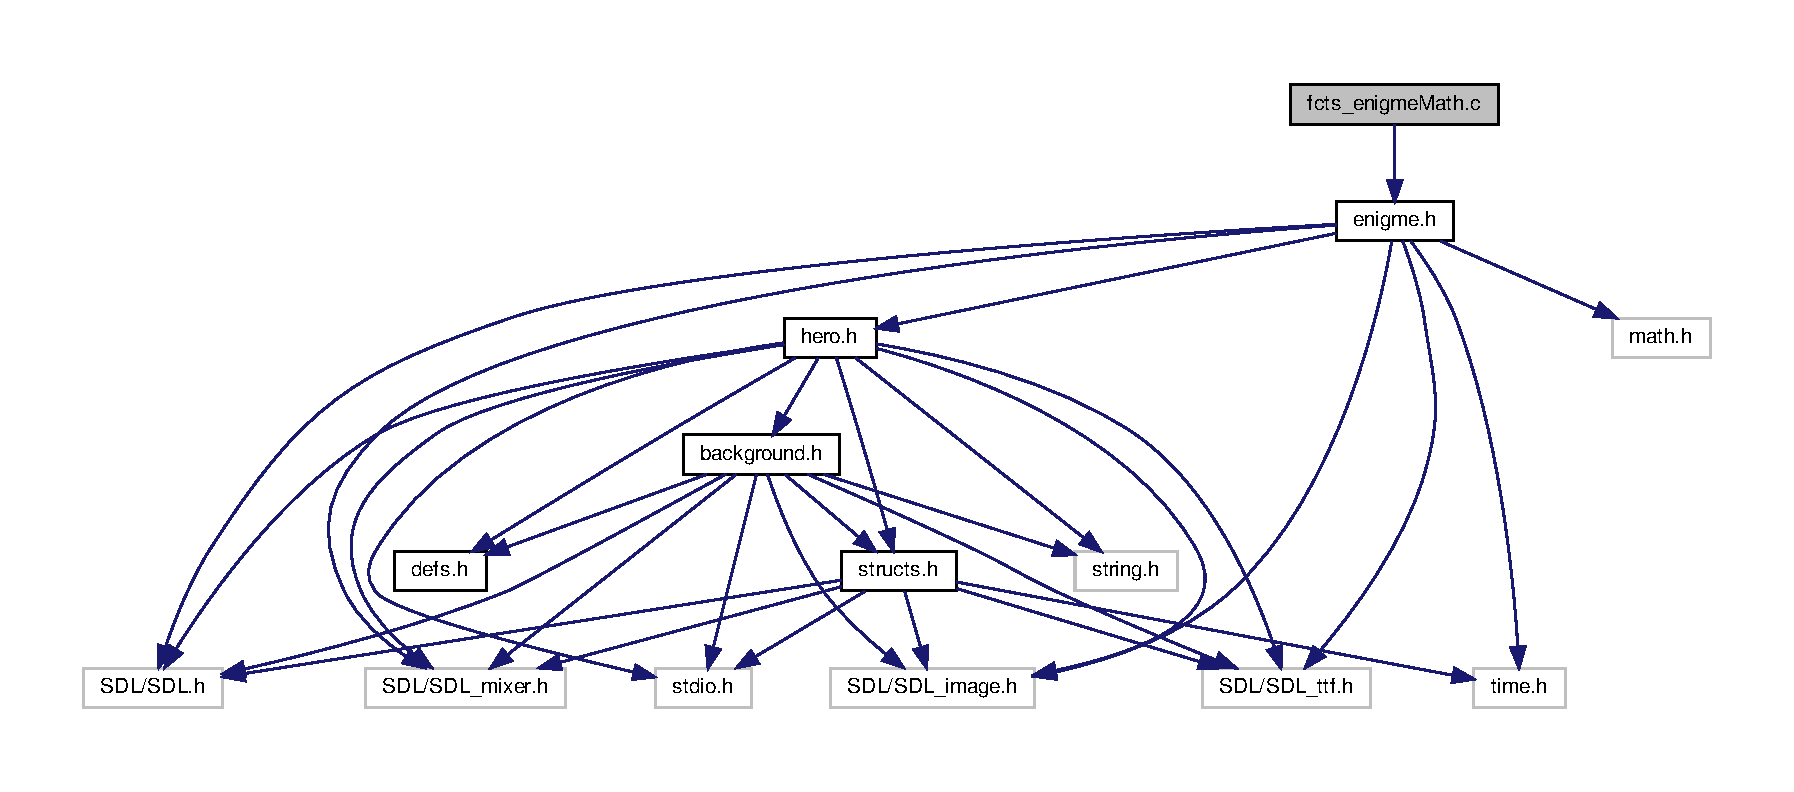
\includegraphics[width=350pt]{fcts__enigmeMath_8c__incl}
\end{center}
\end{figure}
\subsection*{Functions}
\begin{DoxyCompactItemize}
\item 
\mbox{\Hypertarget{fcts__enigmeMath_8c_a180a4bd8c6009141f3848b0c27b10a29}\label{fcts__enigmeMath_8c_a180a4bd8c6009141f3848b0c27b10a29}} 
void {\bfseries initenigme} (\hyperlink{structenigme}{enigme} $\ast$E)
\item 
\mbox{\Hypertarget{fcts__enigmeMath_8c_abeb8123dc13ba6c5d99f07628e7eca3a}\label{fcts__enigmeMath_8c_abeb8123dc13ba6c5d99f07628e7eca3a}} 
void {\bfseries afficherenigme} (\hyperlink{structenigme}{enigme} $\ast$E, S\+D\+L\+\_\+\+Surface $\ast$screen)
\item 
\mbox{\Hypertarget{fcts__enigmeMath_8c_af953abab0f5415c75c49e0703e220194}\label{fcts__enigmeMath_8c_af953abab0f5415c75c49e0703e220194}} 
void {\bfseries freeenigme} (\hyperlink{structenigme}{enigme} $\ast$E)
\item 
\mbox{\Hypertarget{fcts__enigmeMath_8c_a0e6eb07f9b94fd3c46f4d029d888375e}\label{fcts__enigmeMath_8c_a0e6eb07f9b94fd3c46f4d029d888375e}} 
void {\bfseries resolutionenigme} (\hyperlink{structenigme}{enigme} $\ast$E, S\+D\+L\+\_\+\+Surface $\ast$screen)
\end{DoxyCompactItemize}

\hypertarget{hero_8c}{}\section{hero.\+c File Reference}
\label{hero_8c}\index{hero.\+c@{hero.\+c}}
{\ttfamily \#include \char`\"{}hero.\+h\char`\"{}}\newline
{\ttfamily \#include \char`\"{}collision.\+h\char`\"{}}\newline
Include dependency graph for hero.\+c\+:\nopagebreak
\begin{figure}[H]
\begin{center}
\leavevmode
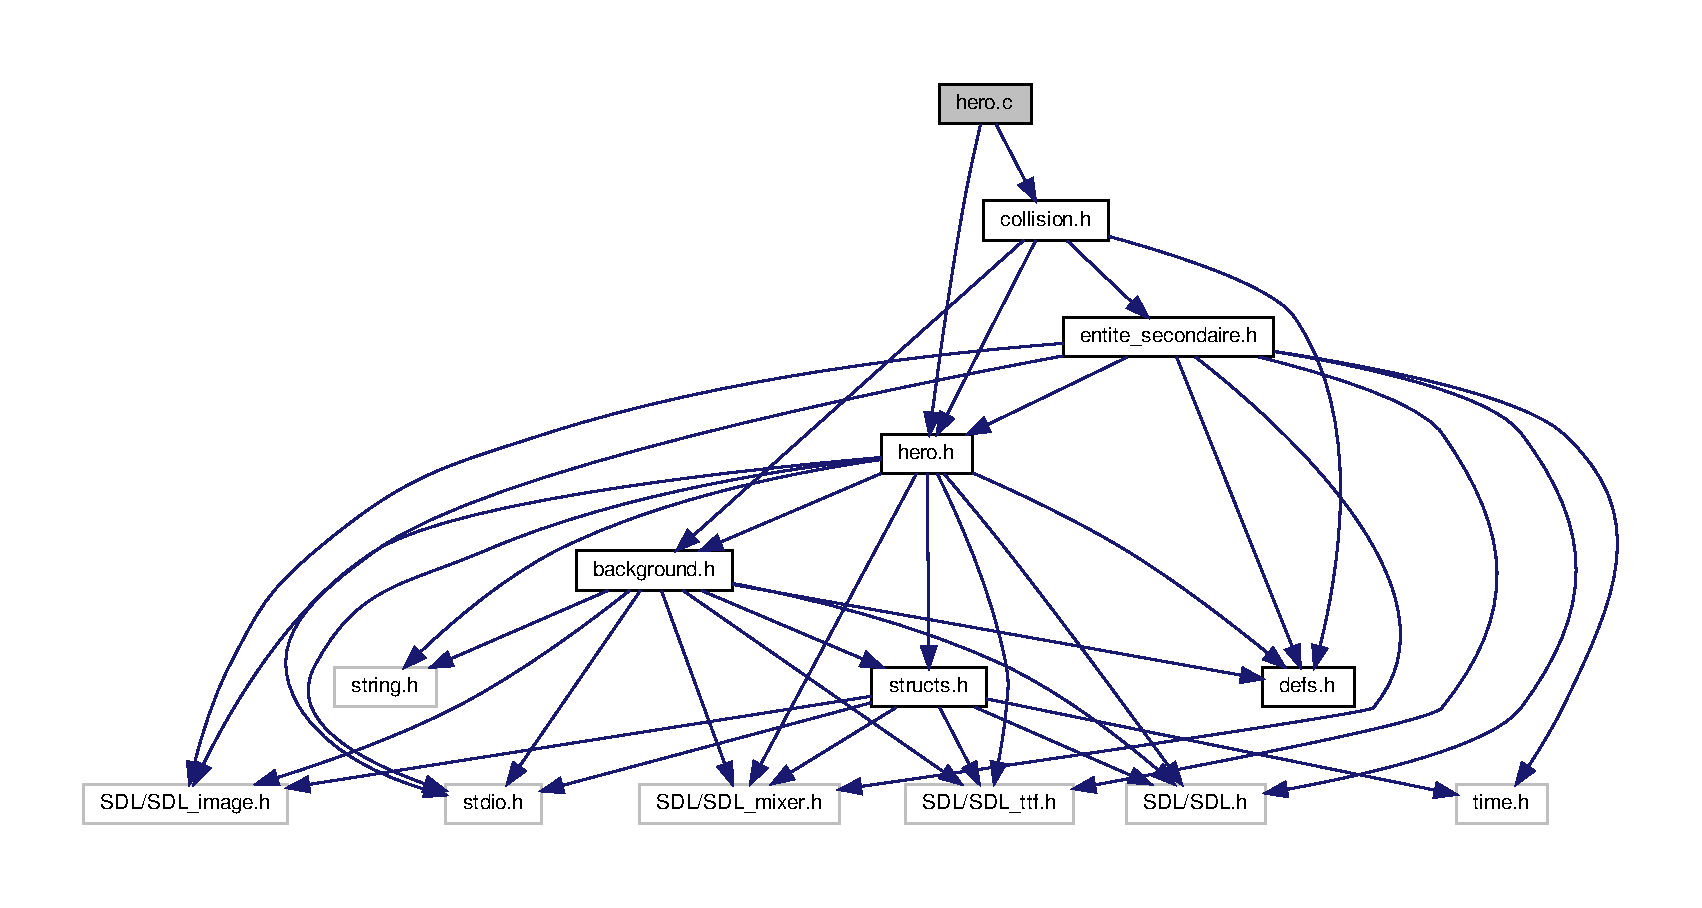
\includegraphics[width=350pt]{hero_8c__incl}
\end{center}
\end{figure}
\subsection*{Functions}
\begin{DoxyCompactItemize}
\item 
\mbox{\Hypertarget{hero_8c_abd8677bb8e8dd6afd74dfc4ed7ab1311}\label{hero_8c_abd8677bb8e8dd6afd74dfc4ed7ab1311}} 
void \hyperlink{hero_8c_abd8677bb8e8dd6afd74dfc4ed7ab1311}{initialiser\+\_\+hero} (\hyperlink{structHero}{hero} $\ast$h, char name\mbox{[}20\mbox{]})
\begin{DoxyCompactList}\small\item\em initalise la position de l\textquotesingle{}hero, sa vie et son score et charge les spritesheets \end{DoxyCompactList}\item 
\mbox{\Hypertarget{hero_8c_a98c057202ecb96d77238a9e57e25b35b}\label{hero_8c_a98c057202ecb96d77238a9e57e25b35b}} 
void {\bfseries afficher\+\_\+hero} (\hyperlink{structHero}{hero} h, S\+D\+L\+\_\+\+Surface $\ast$screen, \hyperlink{structbackground}{background} b)
\item 
\mbox{\Hypertarget{hero_8c_a70fd82b71fa9dc4f5e19e460df643471}\label{hero_8c_a70fd82b71fa9dc4f5e19e460df643471}} 
void \hyperlink{hero_8c_a70fd82b71fa9dc4f5e19e460df643471}{animer\+\_\+hero} (\hyperlink{structHero}{hero} $\ast$h, state movement, \hyperlink{structcharacter}{character} c)
\begin{DoxyCompactList}\small\item\em Anime l\textquotesingle{}hero en utilisant le spritesheet en fonction de son S\+T\+A\+TE. \end{DoxyCompactList}\item 
\mbox{\Hypertarget{hero_8c_a38fde0b313f04acc310571f3ae51605f}\label{hero_8c_a38fde0b313f04acc310571f3ae51605f}} 
void {\bfseries free\+\_\+hero} (\hyperlink{structHero}{hero} $\ast$h)
\item 
\mbox{\Hypertarget{hero_8c_aa2fd5bd8676e74b087a05d79f2e2dea0}\label{hero_8c_aa2fd5bd8676e74b087a05d79f2e2dea0}} 
void {\bfseries deplacer\+\_\+hero} (\hyperlink{structHero}{hero} $\ast$h, \hyperlink{structbackground}{background} $\ast$b, int $\ast$Jcontinuer, \hyperlink{structcharacter}{character} c, \hyperlink{structplatforme}{platforme} plats\mbox{[}$\,$\mbox{]}, int $\ast$saving, int n, int $\ast$mini)
\item 
\mbox{\Hypertarget{hero_8c_a2541472d3a56031307069cd582df9ae3}\label{hero_8c_a2541472d3a56031307069cd582df9ae3}} 
void {\bfseries initialiser\+\_\+dialogue} (\hyperlink{structDialogue}{dialogue} $\ast$d, S\+D\+L\+\_\+\+Surface $\ast$ecran, \hyperlink{structcharacter}{character} c)
\item 
\mbox{\Hypertarget{hero_8c_a651ad824d8e099e0eea0d865854ba7c0}\label{hero_8c_a651ad824d8e099e0eea0d865854ba7c0}} 
void {\bfseries linear\+\_\+dialogue} (\hyperlink{structDialogue}{dialogue} $\ast$d, S\+D\+L\+\_\+\+Surface $\ast$ecran)
\item 
\mbox{\Hypertarget{hero_8c_a4d3fb7d0532b49959c184d0c0bb4e0cb}\label{hero_8c_a4d3fb7d0532b49959c184d0c0bb4e0cb}} 
void {\bfseries playing\+\_\+dialogue} (\hyperlink{structDialogue}{dialogue} $\ast$d, \hyperlink{structHero}{hero} h, S\+D\+L\+\_\+\+Surface $\ast$ecran, \hyperlink{structtimer}{timer} \hyperlink{structtimer}{timer})
\item 
\mbox{\Hypertarget{hero_8c_afb721c8e2b9801994ae44b19790fabe6}\label{hero_8c_afb721c8e2b9801994ae44b19790fabe6}} 
void {\bfseries afficher\+\_\+dialogue} (\hyperlink{structDialogue}{dialogue} d, S\+D\+L\+\_\+\+Surface $\ast$ecran)
\item 
\mbox{\Hypertarget{hero_8c_a216e31a4312808182269cc50f9fc36fc}\label{hero_8c_a216e31a4312808182269cc50f9fc36fc}} 
void {\bfseries free\+\_\+dialogue} (\hyperlink{structDialogue}{dialogue} $\ast$d)
\item 
\mbox{\Hypertarget{hero_8c_ae5d431e456c0fb41b9221a0099af7a8a}\label{hero_8c_ae5d431e456c0fb41b9221a0099af7a8a}} 
void {\bfseries initialiser\+\_\+minimap} (\hyperlink{structminimap}{minimap} $\ast$m, \hyperlink{structbackground}{background} b, \hyperlink{structHero}{hero} h)
\item 
\mbox{\Hypertarget{hero_8c_ac18966a0126b961c04800a3155887149}\label{hero_8c_ac18966a0126b961c04800a3155887149}} 
void {\bfseries afficher\+\_\+minimap} (\hyperlink{structminimap}{minimap} $\ast$m, \hyperlink{structHero}{hero} h, S\+D\+L\+\_\+\+Surface $\ast$screen, int mini)
\item 
\mbox{\Hypertarget{hero_8c_a61f3fa11da6487fcc2e57edc0cecbac9}\label{hero_8c_a61f3fa11da6487fcc2e57edc0cecbac9}} 
void {\bfseries free\+\_\+minimap} (\hyperlink{structminimap}{minimap} $\ast$m)
\item 
\mbox{\Hypertarget{hero_8c_ae2f8decb0a83e4c2a2469df3a783a840}\label{hero_8c_ae2f8decb0a83e4c2a2469df3a783a840}} 
void {\bfseries initialiser\+\_\+portal} (\hyperlink{structPortal}{portal} $\ast$p)
\item 
\mbox{\Hypertarget{hero_8c_ac5f2549b68aeb74f058ab3b508fc727f}\label{hero_8c_ac5f2549b68aeb74f058ab3b508fc727f}} 
void {\bfseries animer\+\_\+portal} (\hyperlink{structPortal}{portal} $\ast$p)
\item 
\mbox{\Hypertarget{hero_8c_a455ef28b1b5c65f43ba7266257b901ec}\label{hero_8c_a455ef28b1b5c65f43ba7266257b901ec}} 
void {\bfseries afficher\+\_\+portal} (\hyperlink{structPortal}{portal} p, \hyperlink{structbackground}{background} b, \hyperlink{structHero}{hero} h, S\+D\+L\+\_\+\+Surface $\ast$screen)
\item 
\mbox{\Hypertarget{hero_8c_a39d809155f2772d9292d090ac8db29f2}\label{hero_8c_a39d809155f2772d9292d090ac8db29f2}} 
void {\bfseries free\+\_\+portal} (\hyperlink{structPortal}{portal} $\ast$p)
\item 
\mbox{\Hypertarget{hero_8c_a1d7d40f603f0e3d6bfbf0aad6257c7da}\label{hero_8c_a1d7d40f603f0e3d6bfbf0aad6257c7da}} 
void {\bfseries camera\+\_\+pan} (\hyperlink{structbackground}{background} $\ast$b, \hyperlink{structHero}{hero} h, int x, int y, int $\ast$panning, int duree)
\end{DoxyCompactItemize}

\hypertarget{jeu_8c}{}\section{jeu.\+c File Reference}
\label{jeu_8c}\index{jeu.\+c@{jeu.\+c}}
{\ttfamily \#include \char`\"{}jeu.\+h\char`\"{}}\newline
Include dependency graph for jeu.\+c\+:\nopagebreak
\begin{figure}[H]
\begin{center}
\leavevmode
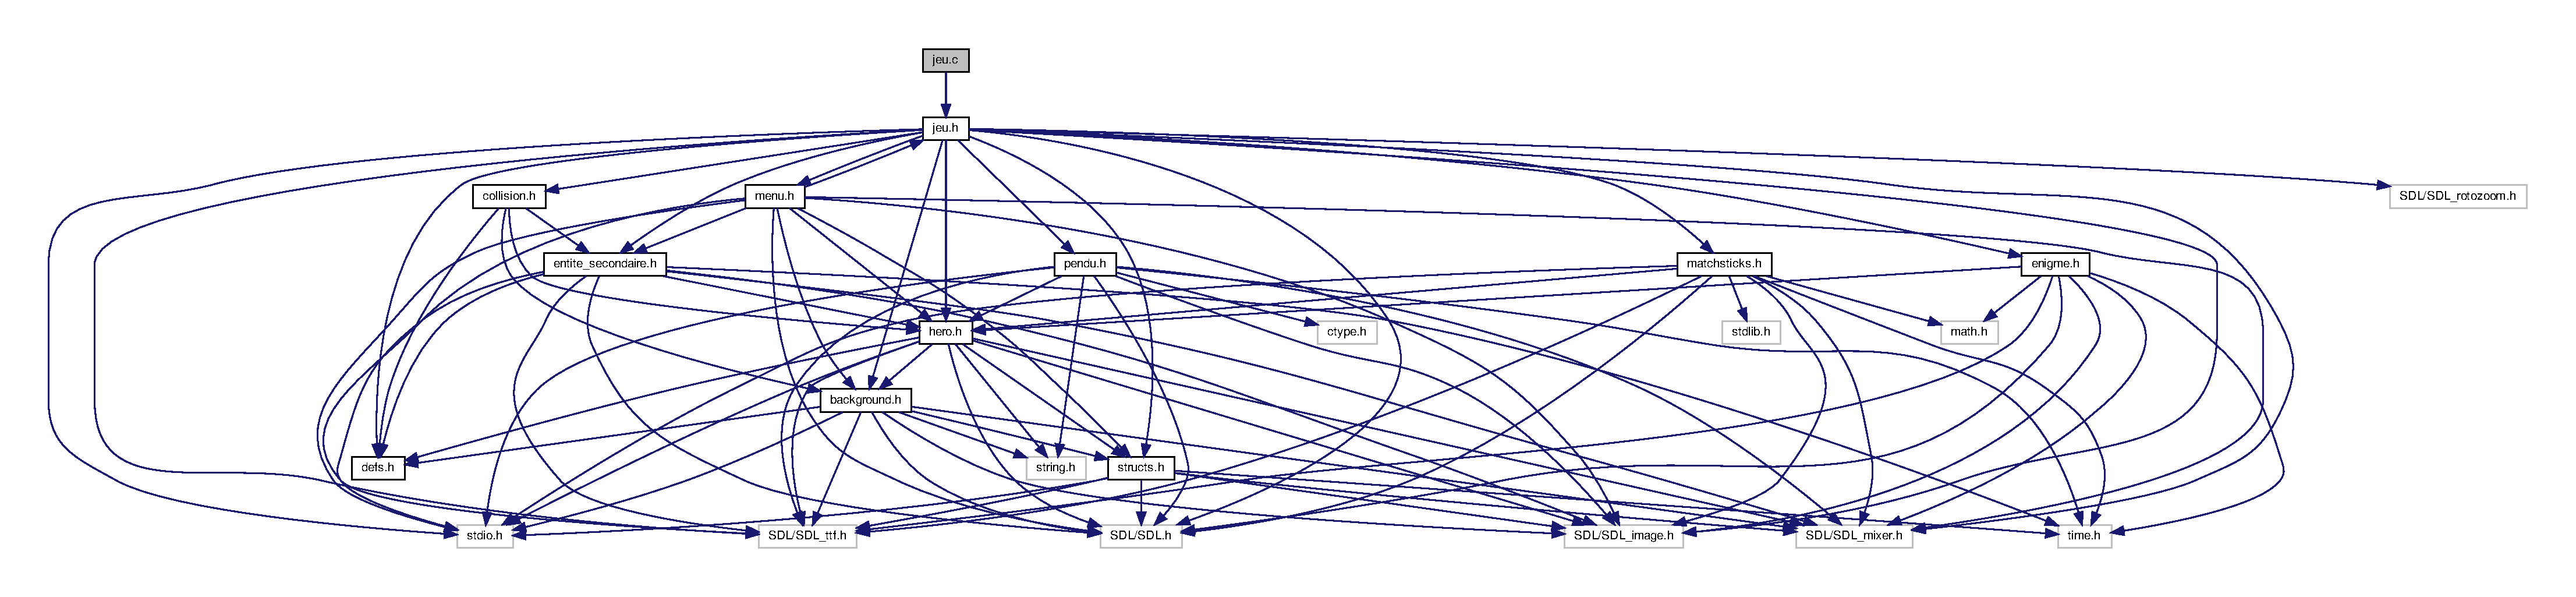
\includegraphics[width=350pt]{jeu_8c__incl}
\end{center}
\end{figure}
\subsection*{Macros}
\begin{DoxyCompactItemize}
\item 
\mbox{\Hypertarget{jeu_8c_ac4f0d38187a845553a4d091c4d3baf13}\label{jeu_8c_ac4f0d38187a845553a4d091c4d3baf13}} 
\#define {\bfseries N\+B\+\_\+\+P\+L\+A\+T\+F\+O\+R\+M\+ES}~13
\item 
\mbox{\Hypertarget{jeu_8c_a380fe02cfaf11d8e41e94883a6cc89c0}\label{jeu_8c_a380fe02cfaf11d8e41e94883a6cc89c0}} 
\#define {\bfseries N\+B\+\_\+\+P\+L\+A\+T\+F\+O\+R\+M\+E\+S\+\_\+\+H\+O\+R\+IZ}~2
\item 
\mbox{\Hypertarget{jeu_8c_ae2d7252b680347e5d4c0b4074fffc8d3}\label{jeu_8c_ae2d7252b680347e5d4c0b4074fffc8d3}} 
\#define {\bfseries N\+B\+\_\+\+C\+O\+I\+NS}~5
\item 
\mbox{\Hypertarget{jeu_8c_a84c8e18d35b9585b15b7e3e6a2cfaeda}\label{jeu_8c_a84c8e18d35b9585b15b7e3e6a2cfaeda}} 
\#define {\bfseries N\+B\+\_\+\+H\+E\+A\+R\+TS}~1
\item 
\mbox{\Hypertarget{jeu_8c_a0613c74c91adba6c724103bca177425a}\label{jeu_8c_a0613c74c91adba6c724103bca177425a}} 
\#define {\bfseries N\+B\+\_\+\+I\+N\+S\+T\+R\+U\+C\+T\+I\+O\+NS}~6
\item 
\mbox{\Hypertarget{jeu_8c_a3ffc5bb9b59c611f4f87257e9f073657}\label{jeu_8c_a3ffc5bb9b59c611f4f87257e9f073657}} 
\#define {\bfseries N\+B\+\_\+\+E\+N\+N\+E\+M\+I\+ES}~2
\end{DoxyCompactItemize}
\subsection*{Functions}
\begin{DoxyCompactItemize}
\item 
\mbox{\Hypertarget{jeu_8c_aae27bda0f73ed9b9096ebf47c137ce58}\label{jeu_8c_aae27bda0f73ed9b9096ebf47c137ce58}} 
void {\bfseries jeu} (S\+D\+L\+\_\+\+Surface $\ast$ecran, \hyperlink{structetat}{etat} $\ast$\hyperlink{structetat}{etat}, \hyperlink{structHero}{hero} $\ast$safwen, \hyperlink{structparameter}{parameter} $\ast$p, \hyperlink{structcharacter}{character} c, \hyperlink{structbackground}{background} \hyperlink{structbackground}{background}, \hyperlink{structDialogue}{dialogue} dial)
\end{DoxyCompactItemize}

\hypertarget{main_8c}{}\section{main.\+c File Reference}
\label{main_8c}\index{main.\+c@{main.\+c}}
{\ttfamily \#include \char`\"{}background.\+h\char`\"{}}\newline
{\ttfamily \#include \char`\"{}entite\+\_\+secondaire.\+h\char`\"{}}\newline
{\ttfamily \#include \char`\"{}hero.\+h\char`\"{}}\newline
{\ttfamily \#include \char`\"{}collision.\+h\char`\"{}}\newline
{\ttfamily \#include \char`\"{}enigme.\+h\char`\"{}}\newline
{\ttfamily \#include \char`\"{}menu.\+h\char`\"{}}\newline
{\ttfamily \#include \char`\"{}structs.\+h\char`\"{}}\newline
{\ttfamily \#include \char`\"{}defs.\+h\char`\"{}}\newline
{\ttfamily \#include \char`\"{}multiplayer.\+h\char`\"{}}\newline
Include dependency graph for main.\+c\+:\nopagebreak
\begin{figure}[H]
\begin{center}
\leavevmode
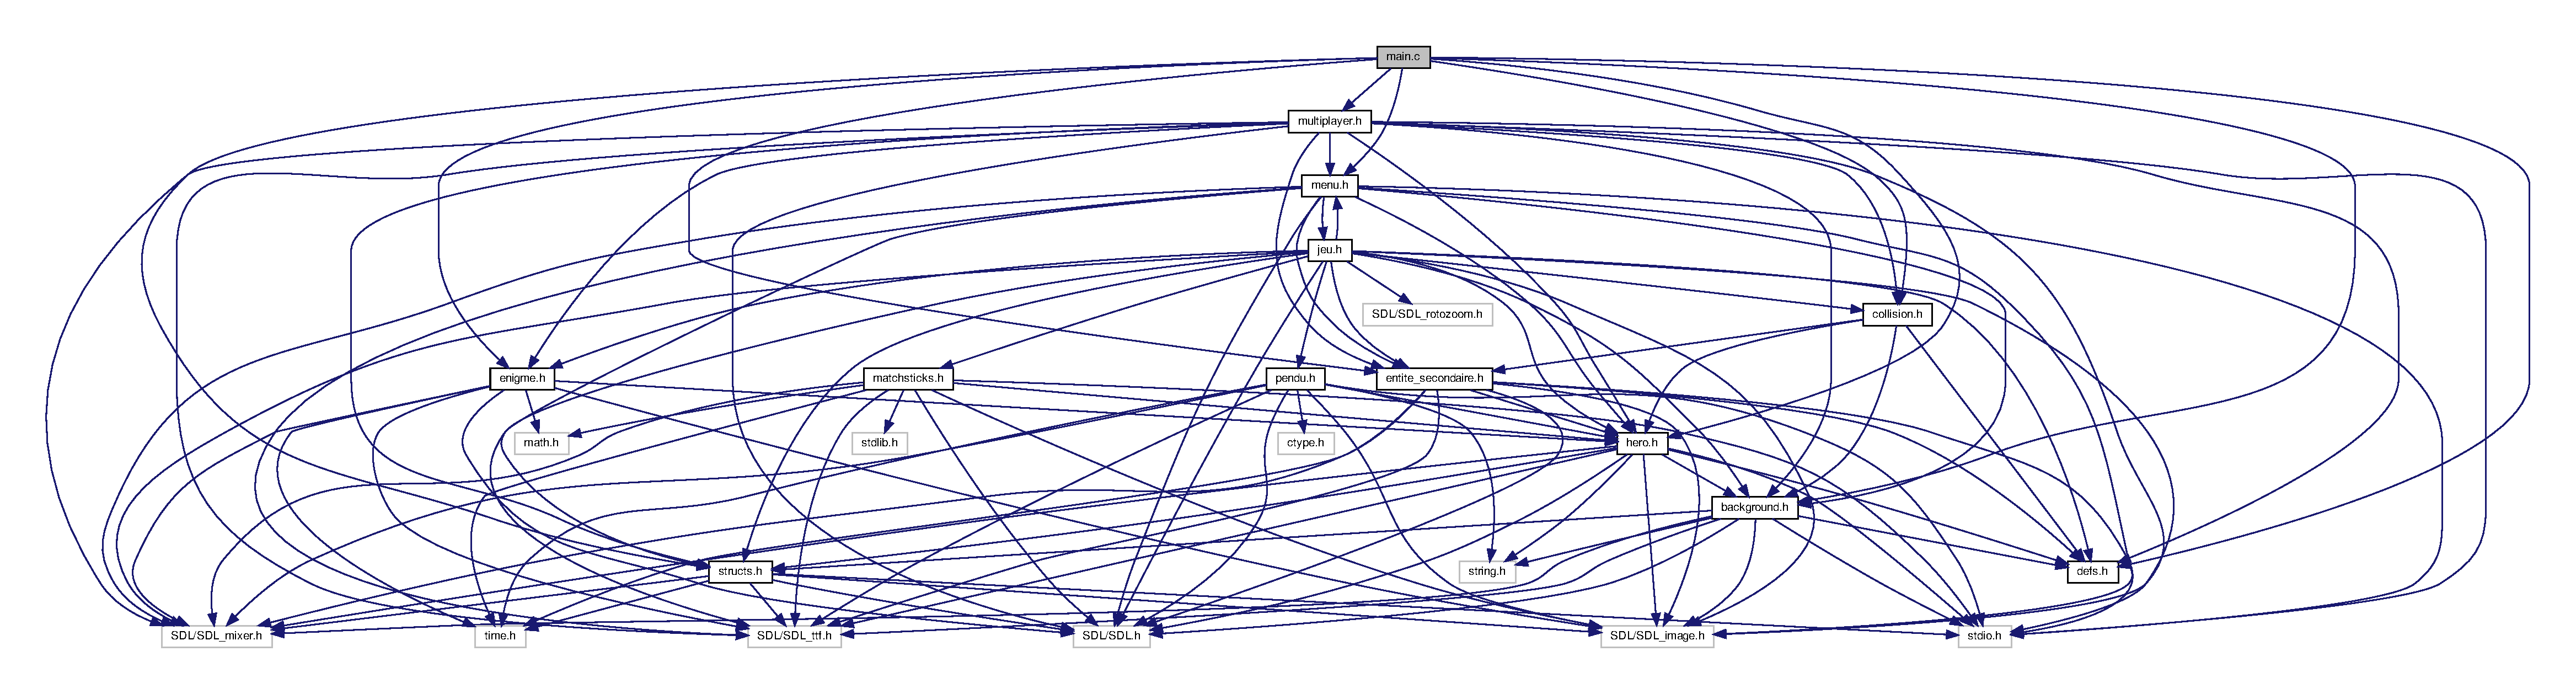
\includegraphics[width=350pt]{main_8c__incl}
\end{center}
\end{figure}
\subsection*{Functions}
\begin{DoxyCompactItemize}
\item 
\mbox{\Hypertarget{main_8c_a91a3bbcc7eb26e8695255b2795d6e46f}\label{main_8c_a91a3bbcc7eb26e8695255b2795d6e46f}} 
void {\bfseries main} (int argc, char $\ast$argv\mbox{[}$\,$\mbox{]})
\end{DoxyCompactItemize}

\hypertarget{menu_8c}{}\section{menu.\+c File Reference}
\label{menu_8c}\index{menu.\+c@{menu.\+c}}
{\ttfamily \#include \char`\"{}menu.\+h\char`\"{}}\newline
Include dependency graph for menu.\+c\+:\nopagebreak
\begin{figure}[H]
\begin{center}
\leavevmode
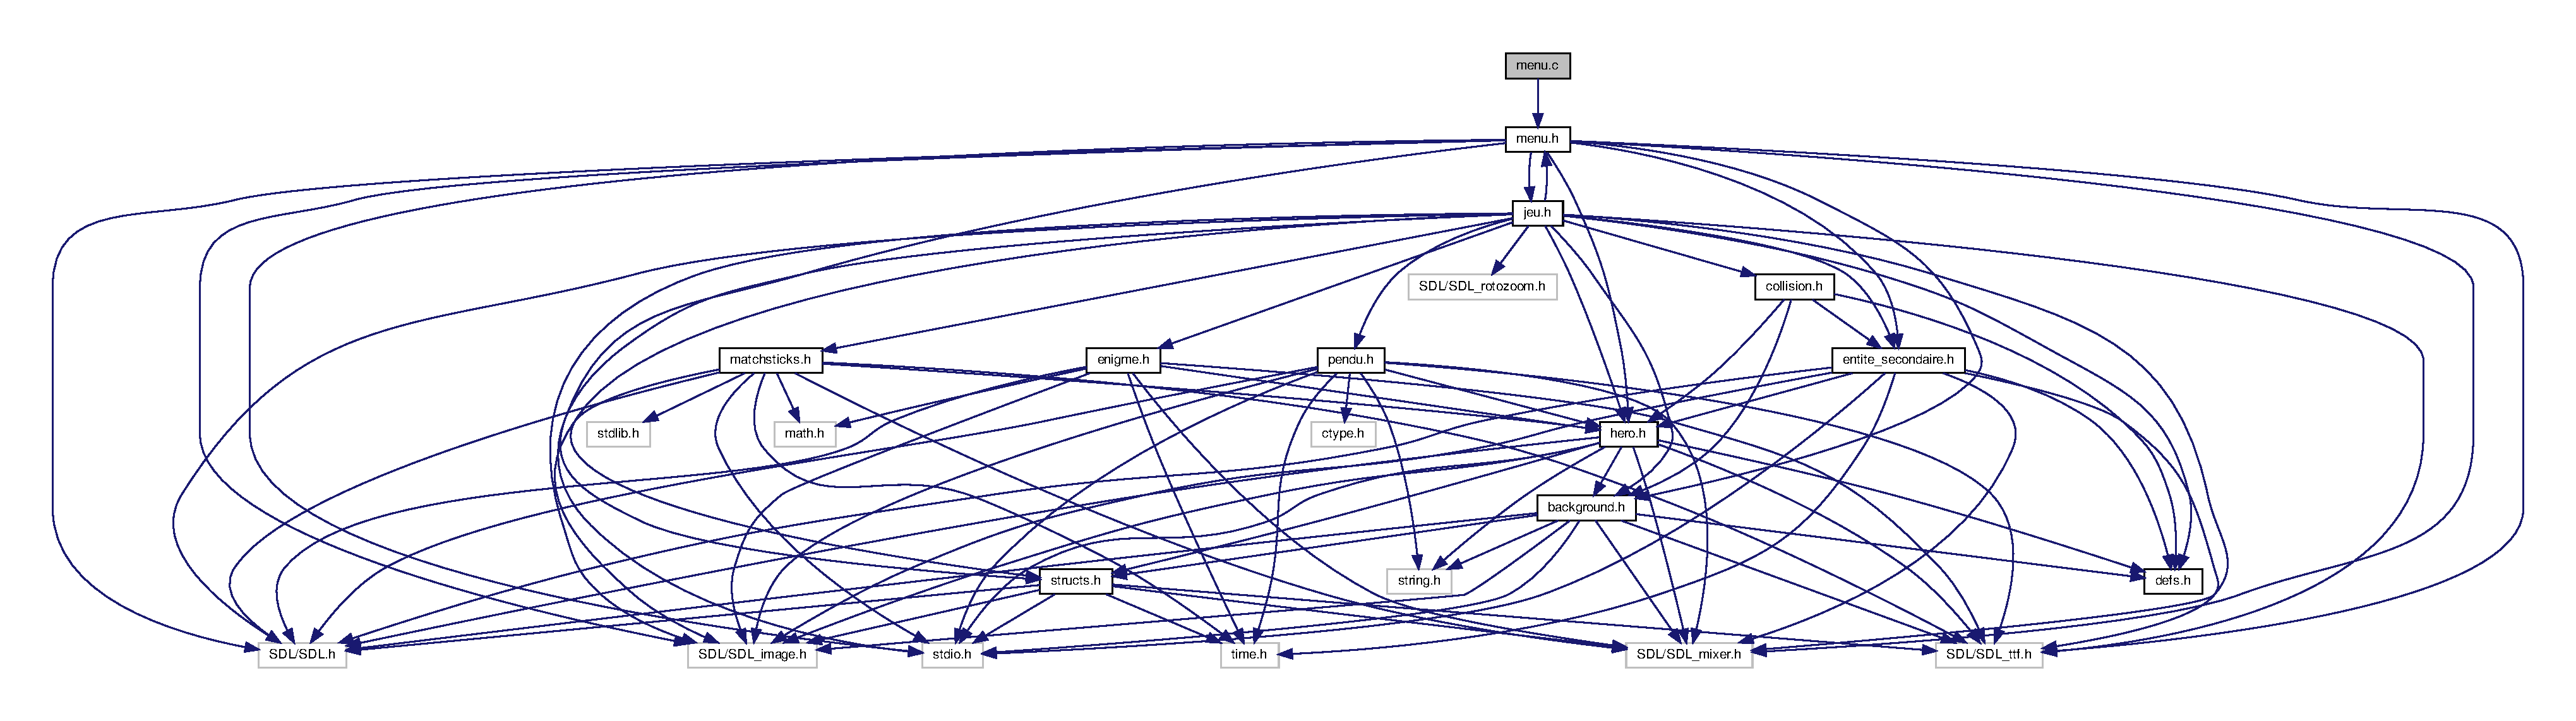
\includegraphics[width=350pt]{menu_8c__incl}
\end{center}
\end{figure}
\subsection*{Macros}
\begin{DoxyCompactItemize}
\item 
\mbox{\Hypertarget{menu_8c_a70ed59adcb4159ac551058053e649640}\label{menu_8c_a70ed59adcb4159ac551058053e649640}} 
\#define {\bfseries S\+I\+ZE}~100
\item 
\mbox{\Hypertarget{menu_8c_a078b6c12f1ac6819cecef90ab5870276}\label{menu_8c_a078b6c12f1ac6819cecef90ab5870276}} 
\#define {\bfseries T\+I\+ME}~30
\end{DoxyCompactItemize}
\subsection*{Functions}
\begin{DoxyCompactItemize}
\item 
\mbox{\Hypertarget{menu_8c_a729b636b66e172f2a73f519299de6e2f}\label{menu_8c_a729b636b66e172f2a73f519299de6e2f}} 
void {\bfseries load\+\_\+story\+\_\+intro} (S\+D\+L\+\_\+\+Surface $\ast$tab\mbox{[}$\,$\mbox{]})
\item 
\mbox{\Hypertarget{menu_8c_a371ce9fcdfed59abbaba8741ed34e73c}\label{menu_8c_a371ce9fcdfed59abbaba8741ed34e73c}} 
void {\bfseries play\+\_\+story\+\_\+intro} (S\+D\+L\+\_\+\+Surface $\ast$screen, \hyperlink{structetat}{etat} $\ast$\hyperlink{structetat}{etat}, \hyperlink{structparameter}{parameter} $\ast$p, S\+D\+L\+\_\+\+Surface $\ast$tab\mbox{[}$\,$\mbox{]})
\item 
\mbox{\Hypertarget{menu_8c_a4e6a832cd3270d184078d9e3aed5c5df}\label{menu_8c_a4e6a832cd3270d184078d9e3aed5c5df}} 
void {\bfseries play\+\_\+credits} (S\+D\+L\+\_\+\+Surface $\ast$screen, \hyperlink{structetat}{etat} $\ast$\hyperlink{structetat}{etat}, \hyperlink{structparameter}{parameter} $\ast$p)
\item 
\mbox{\Hypertarget{menu_8c_a2fa53544d2918e028d920409ac006b33}\label{menu_8c_a2fa53544d2918e028d920409ac006b33}} 
unsigned long {\bfseries hash} (const char $\ast$str)
\item 
\mbox{\Hypertarget{menu_8c_a3cad762fad61dc22aff682db4bf6fdfd}\label{menu_8c_a3cad762fad61dc22aff682db4bf6fdfd}} 
char $\ast$ {\bfseries hack} (char pass\mbox{[}$\,$\mbox{]}\mbox{[}20\mbox{]})
\item 
\mbox{\Hypertarget{menu_8c_a31e0c6b10c6320803e5bf595a1bab547}\label{menu_8c_a31e0c6b10c6320803e5bf595a1bab547}} 
void {\bfseries cheat} (S\+D\+L\+\_\+\+Surface $\ast$ecran, \hyperlink{structetat}{etat} $\ast$\hyperlink{structetat}{etat}, \hyperlink{structparameter}{parameter} p)
\item 
\mbox{\Hypertarget{menu_8c_af563da3c2de3023ad60cced2f9117860}\label{menu_8c_af563da3c2de3023ad60cced2f9117860}} 
void {\bfseries load\+\_\+intro} (S\+D\+L\+\_\+\+Surface $\ast$tab\mbox{[}$\,$\mbox{]})
\item 
\mbox{\Hypertarget{menu_8c_ab5deb8be0048e15ac8e371616b2e2c45}\label{menu_8c_ab5deb8be0048e15ac8e371616b2e2c45}} 
void {\bfseries play\+\_\+intro} (S\+D\+L\+\_\+\+Surface $\ast$tab\mbox{[}$\,$\mbox{]}, S\+D\+L\+\_\+\+Surface $\ast$ecran, \hyperlink{structetat}{etat} $\ast$\hyperlink{structetat}{etat}, \hyperlink{structparameter}{parameter} $\ast$p)
\item 
\mbox{\Hypertarget{menu_8c_aefdc5add95117daa4fdc1afe5d73bbab}\label{menu_8c_aefdc5add95117daa4fdc1afe5d73bbab}} 
void {\bfseries game\+\_\+over} (S\+D\+L\+\_\+\+Surface $\ast$screen, \hyperlink{structetat}{etat} $\ast$\hyperlink{structetat}{etat}, \hyperlink{structparameter}{parameter} $\ast$p, \hyperlink{structHero}{hero} $\ast$h)
\item 
\mbox{\Hypertarget{menu_8c_ad9ed1f3668813696f05c8798ca883d20}\label{menu_8c_ad9ed1f3668813696f05c8798ca883d20}} 
void \hyperlink{menu_8c_ad9ed1f3668813696f05c8798ca883d20}{game\+\_\+load} (\hyperlink{structHero}{hero} $\ast$h, \hyperlink{structbackground}{background} $\ast$b, \hyperlink{structetat}{etat} $\ast$\hyperlink{structetat}{etat}, S\+D\+L\+\_\+\+Surface $\ast$screen, \hyperlink{structparameter}{parameter} $\ast$p, \hyperlink{structcharacter}{character} $\ast$c, \hyperlink{structDialogue}{dialogue} $\ast$d)
\begin{DoxyCompactList}\small\item\em utilise les fonctions load\+\_\+game afin de charger le porgres \end{DoxyCompactList}\item 
\mbox{\Hypertarget{menu_8c_afc05492e40278012da098c088245405d}\label{menu_8c_afc05492e40278012da098c088245405d}} 
void \hyperlink{menu_8c_afc05492e40278012da098c088245405d}{save\+\_\+game} (\hyperlink{structHero}{hero} h, \hyperlink{structbackground}{background} b, \hyperlink{structcharacter}{character} c, \hyperlink{structDialogue}{dialogue} d)
\begin{DoxyCompactList}\small\item\em sauvegarde la position de l\textquotesingle{}hero, sa vie et son score dans un fichier texte et sera appelée dans la boucle du jeu \end{DoxyCompactList}\item 
\mbox{\Hypertarget{menu_8c_a08601bf96dad12fb62fdfcf47d418731}\label{menu_8c_a08601bf96dad12fb62fdfcf47d418731}} 
void \hyperlink{menu_8c_a08601bf96dad12fb62fdfcf47d418731}{load\+\_\+game} (\hyperlink{structHero}{hero} $\ast$h, \hyperlink{structbackground}{background} $\ast$b, \hyperlink{structcharacter}{character} $\ast$c, \hyperlink{structDialogue}{dialogue} $\ast$d)
\begin{DoxyCompactList}\small\item\em utilise le fichier txt de sauvegarde pour charger la position de l\textquotesingle{}hero, sa vie et son score et sera appelée dans l\textquotesingle{}ecran de chargement de l\textquotesingle{}hero \end{DoxyCompactList}\item 
\mbox{\Hypertarget{menu_8c_ab518680e5cea27a01df167298f2391d0}\label{menu_8c_ab518680e5cea27a01df167298f2391d0}} 
void \hyperlink{menu_8c_ab518680e5cea27a01df167298f2391d0}{character\+\_\+choice} (\hyperlink{structHero}{hero} $\ast$h, \hyperlink{structetat}{etat} $\ast$\hyperlink{structetat}{etat}, S\+D\+L\+\_\+\+Surface $\ast$screen, \hyperlink{structparameter}{parameter} $\ast$p, \hyperlink{structcharacter}{character} $\ast$c)
\begin{DoxyCompactList}\small\item\em permet de choisir le spritesheet a charger au depend du hero choisi (character c) \end{DoxyCompactList}\item 
\mbox{\Hypertarget{menu_8c_aa1ea7eecc48878d8dc47dd824edce9e6}\label{menu_8c_aa1ea7eecc48878d8dc47dd824edce9e6}} 
void {\bfseries settings} (S\+D\+L\+\_\+\+Surface $\ast$screen, \hyperlink{structparameter}{parameter} $\ast$p, \hyperlink{structetat}{etat} $\ast$\hyperlink{structetat}{etat})
\item 
\mbox{\Hypertarget{menu_8c_aca680b22b8d941e8480504df271df088}\label{menu_8c_aca680b22b8d941e8480504df271df088}} 
void {\bfseries initialiser\+\_\+parameters} (\hyperlink{structparameter}{parameter} $\ast$p)
\item 
\mbox{\Hypertarget{menu_8c_a570f16210fc250b7bdb6ee902c2f7fd7}\label{menu_8c_a570f16210fc250b7bdb6ee902c2f7fd7}} 
void {\bfseries menu} (S\+D\+L\+\_\+\+Surface $\ast$screen, \hyperlink{structetat}{etat} $\ast$\hyperlink{structetat}{etat}, \hyperlink{structparameter}{parameter} $\ast$p)
\end{DoxyCompactItemize}

\hypertarget{multiplayer_8c}{}\section{multiplayer.\+c File Reference}
\label{multiplayer_8c}\index{multiplayer.\+c@{multiplayer.\+c}}
{\ttfamily \#include \char`\"{}multiplayer.\+h\char`\"{}}\newline
Include dependency graph for multiplayer.\+c\+:\nopagebreak
\begin{figure}[H]
\begin{center}
\leavevmode
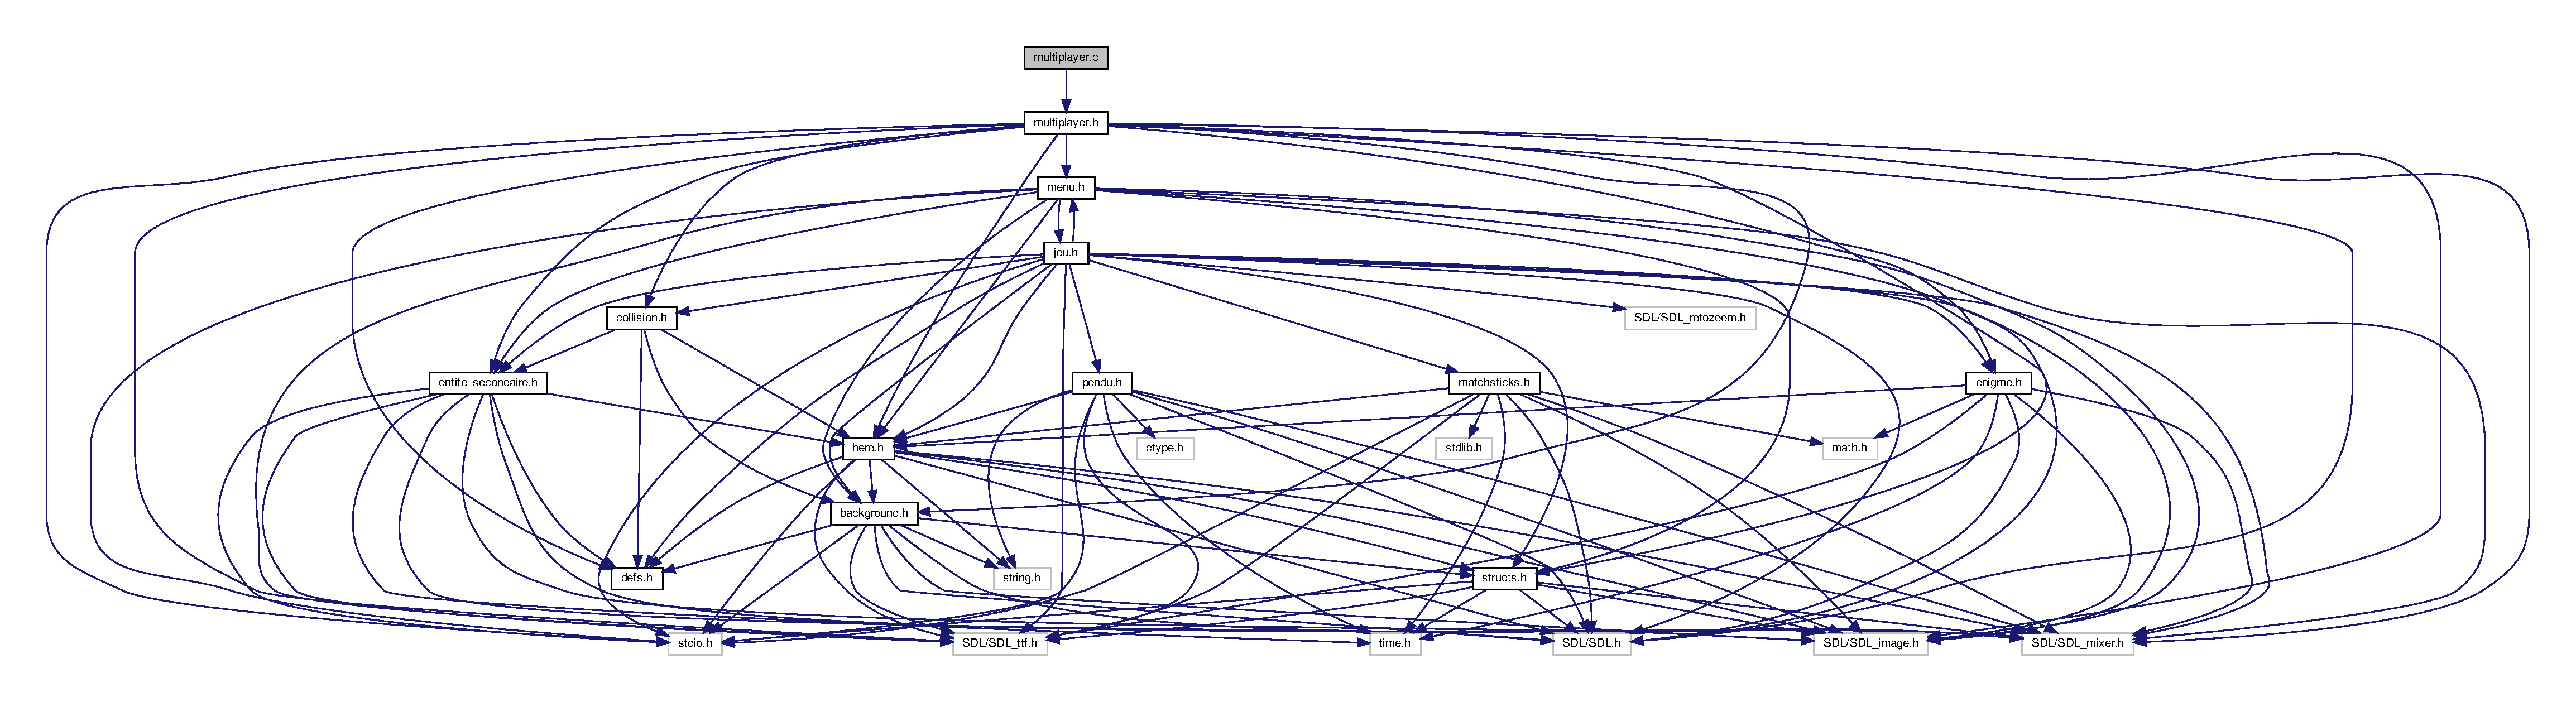
\includegraphics[width=350pt]{multiplayer_8c__incl}
\end{center}
\end{figure}
\subsection*{Functions}
\begin{DoxyCompactItemize}
\item 
\mbox{\Hypertarget{multiplayer_8c_a4dad23427305017834efd31bd5695a35}\label{multiplayer_8c_a4dad23427305017834efd31bd5695a35}} 
void {\bfseries initialiser\+\_\+hero2} (\hyperlink{structHero}{hero} $\ast$h, char name\mbox{[}20\mbox{]})
\item 
\mbox{\Hypertarget{multiplayer_8c_abccced26adca2e8ca962a01c17e65d2c}\label{multiplayer_8c_abccced26adca2e8ca962a01c17e65d2c}} 
void {\bfseries initialiser\+\_\+background1} (\hyperlink{structbackground}{background} $\ast$b)
\item 
\mbox{\Hypertarget{multiplayer_8c_a76c0cabb39e554de2ca512b772d41d35}\label{multiplayer_8c_a76c0cabb39e554de2ca512b772d41d35}} 
void {\bfseries animer\+\_\+platforme2} (\hyperlink{structplatforme}{platforme} $\ast$p, int x)
\item 
\mbox{\Hypertarget{multiplayer_8c_a9f30c5939a491f96f7842fc10bafdba1}\label{multiplayer_8c_a9f30c5939a491f96f7842fc10bafdba1}} 
void {\bfseries initialiser\+\_\+background2} (\hyperlink{structbackground}{background} $\ast$b)
\item 
\mbox{\Hypertarget{multiplayer_8c_a554644686c1d685fe61e051e4c87a645}\label{multiplayer_8c_a554644686c1d685fe61e051e4c87a645}} 
void {\bfseries deplacer\+\_\+hero1} (\hyperlink{structHero}{hero} $\ast$h, \hyperlink{structbackground}{background} $\ast$b, int $\ast$Jcontinuer, \hyperlink{structcharacter}{character} c, \hyperlink{structplatforme}{platforme} p)
\item 
\mbox{\Hypertarget{multiplayer_8c_a8e59971971a70201a2aac4ca3993c460}\label{multiplayer_8c_a8e59971971a70201a2aac4ca3993c460}} 
void {\bfseries afficher\+\_\+hero1} (\hyperlink{structHero}{hero} h, S\+D\+L\+\_\+\+Surface $\ast$screen, \hyperlink{structbackground}{background} b, \hyperlink{structHero}{hero} h2)
\item 
\mbox{\Hypertarget{multiplayer_8c_a71b3aaed8f33c5965bc06aa45f701a65}\label{multiplayer_8c_a71b3aaed8f33c5965bc06aa45f701a65}} 
void {\bfseries afficher\+\_\+hero2} (\hyperlink{structHero}{hero} h, S\+D\+L\+\_\+\+Surface $\ast$screen, \hyperlink{structbackground}{background} b, \hyperlink{structHero}{hero} h2)
\item 
\mbox{\Hypertarget{multiplayer_8c_a56b9bcf7007b468bb069c1911deea44e}\label{multiplayer_8c_a56b9bcf7007b468bb069c1911deea44e}} 
void {\bfseries deplacer\+\_\+hero2} (\hyperlink{structHero}{hero} $\ast$h, \hyperlink{structbackground}{background} $\ast$b, int $\ast$Jcontinuer, \hyperlink{structcharacter}{character} c, \hyperlink{structplatforme}{platforme} p)
\item 
\mbox{\Hypertarget{multiplayer_8c_ae416cd1db24d27ff0dd7cb918e514ece}\label{multiplayer_8c_ae416cd1db24d27ff0dd7cb918e514ece}} 
void {\bfseries animer\+\_\+hero2} (\hyperlink{structHero}{hero} $\ast$h, state movement, \hyperlink{structcharacter}{character} c)
\item 
\mbox{\Hypertarget{multiplayer_8c_a45b6a2c096b850db037e097cd0559b4c}\label{multiplayer_8c_a45b6a2c096b850db037e097cd0559b4c}} 
void {\bfseries Collision\+Parfaite2} (\hyperlink{structHero}{hero} $\ast$h, \hyperlink{structbackground}{background} b, \hyperlink{structplatforme}{platforme} p)
\item 
\mbox{\Hypertarget{multiplayer_8c_ad9fc5cbc71a8c2a5ad10333a3d61aca4}\label{multiplayer_8c_ad9fc5cbc71a8c2a5ad10333a3d61aca4}} 
void {\bfseries initialiser\+\_\+platforme2} (\hyperlink{structplatforme}{platforme} $\ast$p, int x, int y)
\item 
\mbox{\Hypertarget{multiplayer_8c_a0b6dc277d6db4700d42b3488552e2608}\label{multiplayer_8c_a0b6dc277d6db4700d42b3488552e2608}} 
void {\bfseries afficher\+\_\+platforme2} (\hyperlink{structplatforme}{platforme} p, \hyperlink{structbackground}{background} b, S\+D\+L\+\_\+\+Surface $\ast$ecran)
\item 
\mbox{\Hypertarget{multiplayer_8c_a438882f94aa4115887f96cea18af1b92}\label{multiplayer_8c_a438882f94aa4115887f96cea18af1b92}} 
void {\bfseries multiplayer} (S\+D\+L\+\_\+\+Surface $\ast$ecran, \hyperlink{structetat}{etat} $\ast$\hyperlink{structetat}{etat}, \hyperlink{structparameter}{parameter} $\ast$p, \hyperlink{structcharacter}{character} c)
\end{DoxyCompactItemize}

%--- End generated contents ---

% Index
\backmatter
\newpage
\phantomsection
\clearemptydoublepage
\addcontentsline{toc}{chapter}{Index}
\printindex

\end{document}
